
% RECOMMENDED %%%%%%%%%%%%%%%%%%%%%%%%%%%%%%%%%%%%%%%%%%%%%%%%%%%
\documentclass[graybox]{svmult}

% choose options for [] as required from the list
% in the Reference Guide

\usepackage{mathptmx}       % selects Times Roman as basic font
\usepackage{helvet}         % selects Helvetica as sans-serif font
\usepackage{courier}        % selects Courier as typewriter font
\usepackage{type1cm}        % activate if the above 3 fonts are
                            % not available on your system
%
\usepackage{makeidx}         % allows index generation
\usepackage{graphicx}        % standard LaTeX graphics tool
                             % when including figure files
\usepackage{multicol}        % used for the two-column index
\usepackage[bottom]{footmisc}% places footnotes at page bottom

% see the list of further useful packages
% in the Reference Guide

\makeindex             % used for the subject index
                       % please use the style svind.ist with
                       % your makeindex program

%%%%%%%%%%%%%%%%%%%%%%%%%%%%%%%%%%%%%%%%%%%%%%%%%%%%%%%%%%%%%%%%%%%%%%%%%%%%%%%%%%%%%%%%%
\usepackage{multirow}
\usepackage{longtable}
\usepackage{float}

\def\entrywithlabel[#1]#2{\parbox{#1}{{\small #2:} \hrulefill}}
\def\entrywithlabelunder[#1]#2{\parbox{#1}{\hrulefill\\[-.75ex]\centerline {#2}}}
\def\entrywithlabelraised[#1]#2{\parbox{#1}{\smash{\raise-1ex\hbox{{\tiny #2}}}\hrulefill}}
\def\boxentry[#1]#2{{\setlength{\fboxsep}{-\fboxrule}\fbox{\parbox{#1}{\smash{\raise-6.5pt\hbox{~{\tiny #2}}}\vspace{2ex}\mbox{}}}}}
\def\boxpar[#1]#2#3{{\setlength{\fboxsep}{-\fboxrule}\fbox{\parbox[][#2][t]{#1}{\mbox{}\\[-.125\baselineskip]\mbox{}~#3}}}}

\usepackage{tikz}
\usetikzlibrary{calc,trees,positioning,arrows,chains,shapes.geometric,%
    decorations.pathreplacing,decorations.pathmorphing,shapes,%
    matrix,shapes.symbols,shapes.arrows}

\tikzset{
>=stealth',
  punktchain/.style={
    rectangle, 
    rounded corners, 
    % fill=black!10,
    draw=black, very thick,
    text width=10em, 
    minimum height=3em, 
    text centered, 
    on chain},
  line/.style={draw, thick, <-},
  element/.style={
    tape,
    top color=white,
    bottom color=blue!50!black!60!,
    minimum width=10em,
    draw=blue!40!black!90, very thick,
    text width=10em, 
    minimum height=3.5em, 
    text centered, 
    on chain},
  every join/.style={->, thick,shorten >=1pt},
  decoration={brace},
  tuborg/.style={decorate},
  tubnode/.style={midway, right=2pt},
}
\tikzset{
>=stealth',
  pequeno/.style={
    rectangle, 
    rounded corners, 
    % fill=black!10,
    draw=black, very thick,
    text width=2em, 
    minimum height=3em, 
    text centered, 
    on chain},
  line/.style={draw, thick, <-},
  element/.style={
    tape,
    top color=white,
    bottom color=blue!50!black!60!,
    minimum width=2em,
    draw=blue!40!black!90, very thick,
    text width=2em, 
    minimum height=3.5em, 
    text centered, 
    on chain},
  every join/.style={->, thick,shorten >=1pt},
  decoration={brace},
  tuborg/.style={decorate},
  tubnode/.style={midway, right=2pt},
}
\tikzset{
>=stealth',
  grande/.style={
    rectangle, 
    rounded corners, 
    % fill=black!10,
    draw=black, very thick,
    text width=20em, 
    minimum height=3em, 
    text centered, 
    on chain},
  line/.style={draw, thick, <-},
  element/.style={
    tape,
    top color=white,
    bottom color=blue!50!black!60!,
    minimum width=20em,
    draw=blue!40!black!90, very thick,
    text width=20em, 
    minimum height=3.5em, 
    text centered, 
    on chain},
  every join/.style={->, thick,shorten >=1pt},
  decoration={brace},
  tuborg/.style={decorate},
  tubnode/.style={midway, right=2pt},
}

\begin{document}

\title*{Quimioterapia de primeira linha}
% Use \titlerunning{Short Title} for an abbreviated version of
% your contribution title if the original one is too long
\author{Francisco Hélder Cavalcante Félix e Juvenia Bezerra Fontenele}
% Use \authorrunning{Short Title} for an abbreviated version of
% your contribution title if the original one is too long
\institute{Francisco Hélder Cavalcante Félix \at Centro Pediátrico do Câncer, Hospital Infantil Albert Sabin, R. Alberto Montezuma, 350, 60410-780, Fortaleza - CE \email{fhcflx@outlook.com}
\and Juvenia Bezerra Fontenele \at Faculdade de Farmácia, Odontologia e Enfermagem, Universidade Federal do Ceará, R. Alexandre Baraúna, 949, 60430-160, Fortaleza - CE %\email{juvenia.fontenele@gmail.com}
}
%
% Use the package "url.sty" to avoid
% problems with special characters
% used in your e-mail or web address
%
\maketitle

\abstract{}

\section{Glioma de baixo grau}
{\let\thefootnote\relax\footnotetext{Versão Junho/2019}}
\textbf{Racional:} num estudo piloto, o grupo de Eric Bouffet mostrou a viabilidade e boa resposta do uso de vimblastina semanal em pacientes com reação à carboplatina. No estudo fase II do The Hospital for Sick Children, a vimblastina foi eficaz em induzir remissão parcial ou completa em 36\% de 51 pacientes com gliomas de baixo grau recorrentes ou progressivos, após esquemas prévios de quimioterapia e/ou radioterapia \cite{doi:10.1002/cncr.21091,doi:10.1200/JCO.2011.34.5843}. Um estudo fase II que incluiu 54 pacientes com gliomas de baixo grau progressivos usou a vimblastina como primeira linha, mostrando resultados aparentemente semelhantes a outros estudos (como o COG-A9952) \cite{lassaletta}. O protocolo original tratou os pacientes por 70 semanas. Nesta adaptação, os pacientes serão tratados por 1 ano (53 semanas), sendo opcional a prorrogação até completar 70 semanas de tratamento.

\textbf{Elegível:} astrocitoma de baixo grau (pilocítico, difuso, outros), oligodendroglioma, ganglioglioma, tumores mistos (oligoastrocitomas, outros), tumores de vias ópticas/hipotálamo (imagem típica, mesmo sem biópsia). Incluir tumores focais de tronco, excluir DIPG, ou tumores difusos de linha média H3K27M+. Pacientes com reação ou contraindicação ao uso de carboplatina; doença recorrente após prévio tratamento com quimioterapia e/ou radioterapia. Alternativa como primeira linha de tratamento. NÃO INICIAR ESTE PROTOCOLO EM CRIANÇAS GRAVEMENTE ENFERMAS.

\textbf{Alternativa:} a conduta expectante é uma opção, uma vez que, via de regra, o crescimento destes tumores é lento e sua progressão demora anos, ou mesmo décadas. Pacientes de maior risco, como aqueles com lesões de vias ópticas ou hipotálamo, síndrome diencefálica ou com lesões de crescimento rápido devem ser tratados sem grande demora. Se possível, uma nova ressecção cirúrgica deve ser avaliada. O protocolo baseado no estudo COG-A9952 (carboplatina e vincristina) pode ser usado como primeira linha. A principal alternativa adjuvante para pacientes com mais de 5 anos e sem NF-1 é a RT local. Pacientes com astrocitomas difusos têm maior risco de transformação maligna após RT.
%\begin{center}
%\begin{tikzpicture}
%  [node distance=.4cm, start chain=going right,]
%    \node[grande, ] (i) {indução};
%    \node[grande, ] (m) {manutenção};
%    \node[pequeno, below of=i, node distance=2cm] (cv) {cv};
%    \node[pequeno, join] (cv) {cv};
%    \node[pequeno, join] (cv) {cv};
%    \node[pequeno, join] (cv) {cv};
%    \node[pequeno, join] (cv) {cv};
%    \node[pequeno, join] (cv) {v};
%    \node[pequeno, join] (cv) {v};
%    \node[pequeno, join] (cv) {cv};
%    \node[pequeno, join] (cv) {cv};
%    \node[pequeno, join] (cv) {cv};
%    \node[pequeno, join] (cv) {cv};
%\end{tikzpicture}
%\end{center}
\cleardoublepage

\noindent{
\entrywithlabel[1\hsize]{\textbf{Nome}}\hfill
\\[0.3cm]
\entrywithlabel[.45\hsize]{\textbf{Peso}}\hfill  \entrywithlabel[.45\hsize]{\textbf{Estatura}}
}

\subsection{Quimioterapia adjuvante: 53 semanas ou 1 ano}
\begin{center}
\begin{table}[H]
\begin{tabular}{p{1,3cm}p{5,3cm}|p{4,7cm}|p{3cm}}
    \hline
    \multicolumn{1}{c|}{\multirow{2}{*}{\textbf{S1}}}&{Vimblastina \(6,0\)mg/m\(^2\)}&{Administrado: (  ) Sim (  ) Não}&{Rubrica}\\
    \multicolumn{1}{c|}{}&{EV em bolo (max 10mg)}&{Data:}&\\
    \hline
    {Exames:}&{Neut(\(>1,5\times10^3\)):}&{Plaq(\(>10^5\)):}&{TGO:}
    \\
    \hline
    \\
    \hline
    \multicolumn{1}{c|}{\multirow{2}{*}{\textbf{S2}}}&{Vimblastina \(6,0\)mg/m\(^2\)}&{Administrado: (  ) Sim (  ) Não}&{Rubrica}\\
    \multicolumn{1}{c|}{}&{EV em bolo (max 10mg)}&{Data:}&\\
    \hline
    \\
    \hline
    \multicolumn{1}{c|}{\multirow{2}{*}{\textbf{S3}}}&{Vimblastina \(6,0\)mg/m\(^2\)}&{Administrado: (  ) Sim (  ) Não}&{Rubrica}\\
    \multicolumn{1}{c|}{}&{EV em bolo (max 10mg)}&{Data:}&\\
    \hline
    \\
    \hline
    \multicolumn{1}{c|}{\multirow{2}{*}{\textbf{S4}}}&{Vimblastina \(6,0\)mg/m\(^2\)}&{Administrado: (  ) Sim (  ) Não}&{Rubrica}\\
    \multicolumn{1}{c|}{}&{EV em bolo (max 10mg)}&{Data:}&\\
    \hline
    \\
    \hline
    \multicolumn{1}{c|}{\multirow{2}{*}{\textbf{S5}}}&{Vimblastina \(6,0\)mg/m\(^2\)}&{Administrado: (  ) Sim (  ) Não}&{Rubrica}\\
    \multicolumn{1}{c|}{}&{EV em bolo (max 10mg)}&{Data:}&\\
    \hline
    {Exames:}&{Neut(\(>1,5\times10^3\)):}&{Plaq(\(>10^5\)):}&{TGO:}
    \\
    \hline\\
    \hline
    \multicolumn{1}{c|}{\multirow{2}{*}{\textbf{S6}}}&{Vimblastina \(6,0\)mg/m\(^2\)}&{Administrado: (  ) Sim (  ) Não}&{Rubrica}\\
    \multicolumn{1}{c|}{}&{EV em bolo (max 10mg)}&{Data:}&\\
    \hline
    \\
    \hline
    \multicolumn{1}{c|}{\multirow{2}{*}{\textbf{S7}}}&{Vimblastina \(6,0\)mg/m\(^2\)}&{Administrado: (  ) Sim (  ) Não}&{Rubrica}\\
    \multicolumn{1}{c|}{}&{EV em bolo (max 10mg)}&{Data:}&\\
    \hline
    \\
    \hline
    \multicolumn{1}{c|}{\multirow{2}{*}{\textbf{S8}}}&{Vimblastina \(6,0\)mg/m\(^2\)}&{Administrado: (  ) Sim (  ) Não}&{Rubrica}\\
    \multicolumn{1}{c|}{}&{EV em bolo (max 10mg)}&{Data:}&\\
    \hline
    \\
    \hline
    \multicolumn{1}{c|}{\multirow{2}{*}{\textbf{S9}}}&{Vimblastina \(6,0\)mg/m\(^2\)}&{Administrado: (  ) Sim (  ) Não}&{Rubrica}\\
    \multicolumn{1}{c|}{}&{EV em bolo (max 10mg)}&{Data:}&\\
    \hline
    {Exames:}&{Neut(\(>1,5\times10^3\)):}&{Plaq(\(>10^5\)):}&{TGO:}
    \\
    \hline
    \\
    \hline
    \multicolumn{1}{c|}{\multirow{2}{*}{\textbf{S10}}}&{Vimblastina \(6,0\)mg/m\(^2\)}&{Administrado: (  ) Sim (  ) Não}&{Rubrica}\\
    \multicolumn{1}{c|}{}&{EV em bolo (max 10mg)}&{Data:}&\\
    \hline
    \\
    \hline
    \multicolumn{1}{c|}{\multirow{2}{*}{\textbf{S11}}}&{Vimblastina \(6,0\)mg/m\(^2\)}&{Administrado: (  ) Sim (  ) Não}&{Rubrica}\\
    \multicolumn{1}{c|}{}&{EV em bolo (max 10mg)}&{Data:}&\\
    \hline
    \\
    \hline
    \multicolumn{1}{c|}{\multirow{2}{*}{\textbf{S12}}}&{Vimblastina \(6,0\)mg/m\(^2\)}&{Administrado: (  ) Sim (  ) Não}&{Rubrica}\\
    \multicolumn{1}{c|}{}&{EV em bolo (max 10mg)}&{Data:}&\\
    \hline
    \\
    \hline
    \multicolumn{1}{c|}{\multirow{2}{*}{\textbf{S13}}}&{Vimblastina \(6,0\)mg/m\(^2\)}&{Administrado: (  ) Sim (  ) Não}&{Rubrica}\\
    \multicolumn{1}{c|}{}&{EV em bolo (max 10mg)}&{Data:}&\\
    \hline
    {Exames:}&{Neut(\(>1,5\times10^3\)):}&{Plaq(\(>10^5\)):}&{TGO:}
    \\
    \hline
\end{tabular}
\end{table}
\begin{table}[H]
\begin{tabular}{p{1,3cm}p{5,3cm}|p{4,7cm}|p{3cm}}
    \hline
    \multicolumn{1}{c|}{\multirow{2}{*}{\textbf{S14}}}&{Vimblastina \(6,0\)mg/m\(^2\)}&{Administrado: (  ) Sim (  ) Não}&{Rubrica}\\
    \multicolumn{1}{c|}{}&{EV em bolo (max 10mg)}&{Data:}&\\
    \hline
    \\
    \hline
    \multicolumn{1}{c|}{\multirow{2}{*}{\textbf{S15}}}&{Vimblastina \(6,0\)mg/m\(^2\)}&{Administrado: (  ) Sim (  ) Não}&{Rubrica}\\
    \multicolumn{1}{c|}{}&{EV em bolo (max 10mg)}&{Data:}&\\
    \hline
    \\
    \hline
    \multicolumn{1}{c|}{\multirow{2}{*}{\textbf{S16}}}&{Vimblastina \(6,0\)mg/m\(^2\)}&{Administrado: (  ) Sim (  ) Não}&{Rubrica}\\
    \multicolumn{1}{c|}{}&{EV em bolo (max 10mg)}&{Data:}&\\
    \hline
    \\
     \hline
    \multicolumn{1}{c|}{\multirow{2}{*}{\textbf{S17}}}&{Vimblastina \(6,0\)mg/m\(^2\)}&{Administrado: (  ) Sim (  ) Não}&{Rubrica}\\
    \multicolumn{1}{c|}{}&{EV em bolo (max 10mg)}&{Data:}&\\
    \hline
    {Exames:}&{Neut(\(>1,5\times10^3\)):}&{Plaq(\(>10^5\)):}&{TGO:}
    \\
    \hline
    \\
    \hline
    \multicolumn{1}{c|}{\multirow{2}{*}{\textbf{S18}}}&{Vimblastina \(6,0\)mg/m\(^2\)}&{Administrado: (  ) Sim (  ) Não}&{Rubrica}\\
    \multicolumn{1}{c|}{}&{EV em bolo (max 10mg)}&{Data:}&\\
    \hline\\
    \hline
    \multicolumn{1}{c|}{\multirow{2}{*}{\textbf{S19}}}&{Vimblastina \(6,0\)mg/m\(^2\)}&{Administrado: (  ) Sim (  ) Não}&{Rubrica}\\
    \multicolumn{1}{c|}{}&{EV em bolo (max 10mg)}&{Data:}&\\
    \hline
    \\
    \hline
    \multicolumn{1}{c|}{\multirow{2}{*}{\textbf{S20}}}&{Vimblastina \(6,0\)mg/m\(^2\)}&{Administrado: (  ) Sim (  ) Não}&{Rubrica}\\
    \multicolumn{1}{c|}{}&{EV em bolo (max 10mg)}&{Data:}&\\
    \hline
    \\
    \hline
    \multicolumn{1}{c|}{\multirow{2}{*}{\textbf{S21}}}&{Vimblastina \(6,0\)mg/m\(^2\)}&{Administrado: (  ) Sim (  ) Não}&{Rubrica}\\
    \multicolumn{1}{c|}{}&{EV em bolo (max 10mg)}&{Data:}&\\
    \hline
    {Exames:}&{Neut(\(>1,5\times10^3\)):}&{Plaq(\(>10^5\)):}&{TGO:}
    \\
    \hline
    \\
    \hline
    \multicolumn{1}{c|}{\multirow{2}{*}{\textbf{S22}}}&{Vimblastina \(6,0\)mg/m\(^2\)}&{Administrado: (  ) Sim (  ) Não}&{Rubrica}\\
    \multicolumn{1}{c|}{}&{EV em bolo (max 10mg)}&{Data:}&\\
    \hline
    \\
    \hline
    \multicolumn{1}{c|}{\multirow{2}{*}{\textbf{S23}}}&{Vimblastina \(6,0\)mg/m\(^2\)}&{Administrado: (  ) Sim (  ) Não}&{Rubrica}\\
    \multicolumn{1}{c|}{}&{EV em bolo (max 10mg)}&{Data:}&\\
    \hline
    \\
    \hline
    \multicolumn{1}{c|}{\multirow{2}{*}{\textbf{S24}}}&{Vimblastina \(6,0\)mg/m\(^2\)}&{Administrado: (  ) Sim (  ) Não}&{Rubrica}\\
    \multicolumn{1}{c|}{}&{EV em bolo (max 10mg)}&{Data:}&\\
    \hline
    \\
    \hline
    \multicolumn{1}{c|}{\multirow{2}{*}{\textbf{S25}}}&{Vimblastina \(6,0\)mg/m\(^2\)}&{Administrado: (  ) Sim (  ) Não}&{Rubrica}\\
    \multicolumn{1}{c|}{}&{EV em bolo (max 10mg)}&{Data:}&\\
    \hline
    {Exames:}&{Neut(\(>1,5\times10^3\)):}&{Plaq(\(>10^5\)):}&{TGO:}
    \\
    \hline
    \\
    \hline
    \multicolumn{1}{c|}{\multirow{2}{*}{\textbf{S26}}}&{Vimblastina \(6,0\)mg/m\(^2\)}&{Administrado: (  ) Sim (  ) Não}&{Rubrica}\\
    \multicolumn{1}{c|}{}&{EV em bolo (max 10mg)}&{Data:}&\\
    \hline
    \multicolumn{4}{c}{Realizar imagem (RM) - não interromper protocolo aguardando resultado}
    \\
    \hline\\
    \hline
    \multicolumn{1}{c|}{\multirow{2}{*}{\textbf{S27}}}&{Vimblastina \(6,0\)mg/m\(^2\)}&{Administrado: (  ) Sim (  ) Não}&{Rubrica}\\
    \multicolumn{1}{c|}{}&{EV em bolo (max 10mg)}&{Data:}&\\
    \hline
    \\
    \hline
    \multicolumn{1}{c|}{\multirow{2}{*}{\textbf{S28}}}&{Vimblastina \(6,0\)mg/m\(^2\)}&{Administrado: (  ) Sim (  ) Não}&{Rubrica}\\
    \multicolumn{1}{c|}{}&{EV em bolo (max 10mg)}&{Data:}&\\
    \hline
\end{tabular}
\end{table}

\noindent{
\entrywithlabel[1\hsize]{\textbf{Nome}}\hfill
\\[0.3cm]
\entrywithlabel[.45\hsize]{\textbf{Peso}}\hfill  \entrywithlabel[.45\hsize]{\textbf{Estatura}}
}

\begin{table}[H]
\begin{tabular}{p{1,3cm}p{5,3cm}|p{4,7cm}|p{3cm}}
    \hline
    \multicolumn{1}{c|}{\multirow{2}{*}{\textbf{S29}}}&{Vimblastina \(6,0\)mg/m\(^2\)}&{Administrado: (  ) Sim (  ) Não}&{Rubrica}\\
    \multicolumn{1}{c|}{}&{EV em bolo (max 10mg)}&{Data:}&\\
    \hline
    {Exames:}&{Neut(\(>1,5\times10^3\)):}&{Plaq(\(>10^5\)):}&{TGO:}
    \\
    \hline
    \\
    \hline
    \multicolumn{1}{c|}{\multirow{2}{*}{\textbf{S30}}}&{Vimblastina \(6,0\)mg/m\(^2\)}&{Administrado: (  ) Sim (  ) Não}&{Rubrica}\\
    \multicolumn{1}{c|}{}&{EV em bolo (max 10mg)}&{Data:}&\\
    \hline
    \\
    \hline
    \multicolumn{1}{c|}{\multirow{2}{*}{\textbf{S31}}}&{Vimblastina \(6,0\)mg/m\(^2\)}&{Administrado: (  ) Sim (  ) Não}&{Rubrica}\\
    \multicolumn{1}{c|}{}&{EV em bolo (max 10mg)}&{Data:}&\\
    \hline
   \\
    \hline
    \multicolumn{1}{c|}{\multirow{2}{*}{\textbf{S32}}}&{Vimblastina \(6,0\)mg/m\(^2\)}&{Administrado: (  ) Sim (  ) Não}&{Rubrica}\\
    \multicolumn{1}{c|}{}&{EV em bolo (max 10mg)}&{Data:}&\\
    \hline
    \\
    \hline
    \multicolumn{1}{c|}{\multirow{2}{*}{\textbf{S33}}}&{Vimblastina \(6,0\)mg/m\(^2\)}&{Administrado: (  ) Sim (  ) Não}&{Rubrica}\\
    \multicolumn{1}{c|}{}&{EV em bolo (max 10mg)}&{Data:}&\\
    \hline
    {Exames:}&{Neut(\(>1,5\times10^3\)):}&{Plaq(\(>10^5\)):}&{TGO:}
    \\
    \hline
    \\
    \hline
    \multicolumn{1}{c|}{\multirow{2}{*}{\textbf{S34}}}&{Vimblastina \(6,0\)mg/m\(^2\)}&{Administrado: (  ) Sim (  ) Não}&{Rubrica}\\
    \multicolumn{1}{c|}{}&{EV em bolo (max 10mg)}&{Data:}&\\
    \hline
    \\
    \hline
    \multicolumn{1}{c|}{\multirow{2}{*}{\textbf{S35}}}&{Vimblastina \(6,0\)mg/m\(^2\)}&{Administrado: (  ) Sim (  ) Não}&{Rubrica}\\
    \multicolumn{1}{c|}{}&{EV em bolo (max 10mg)}&{Data:}&\\
    \hline
    \\
    \hline
    \multicolumn{1}{c|}{\multirow{2}{*}{\textbf{S36}}}&{Vimblastina \(6,0\)mg/m\(^2\)}&{Administrado: (  ) Sim (  ) Não}&{Rubrica}\\
    \multicolumn{1}{c|}{}&{EV em bolo (max 10mg)}&{Data:}&\\
    \hline
    \\
        \hline
    \multicolumn{1}{c|}{\multirow{2}{*}{\textbf{S37}}}&{Vimblastina \(6,0\)mg/m\(^2\)}&{Administrado: (  ) Sim (  ) Não}&{Rubrica}\\
    \multicolumn{1}{c|}{}&{EV em bolo (max 10mg)}&{Data:}&\\
    \hline
    {Exames:}&{Neut(\(>1,5\times10^3\)):}&{Plaq(\(>10^5\)):}&{TGO:}
    \\
    \hline
    \\
    \hline
    \multicolumn{1}{c|}{\multirow{2}{*}{\textbf{S38}}}&{Vimblastina \(6,0\)mg/m\(^2\)}&{Administrado: (  ) Sim (  ) Não}&{Rubrica}\\
    \multicolumn{1}{c|}{}&{EV em bolo (max 10mg)}&{Data:}&\\
    \hline
    \\
    \hline
    \multicolumn{1}{c|}{\multirow{2}{*}{\textbf{S39}}}&{Vimblastina \(6,0\)mg/m\(^2\)}&{Administrado: (  ) Sim (  ) Não}&{Rubrica}\\
    \multicolumn{1}{c|}{}&{EV em bolo (max 10mg)}&{Data:}&\\
   \hline
   \multicolumn{4}{c}{Realizar imagem (RM) - não interromper protocolo aguardando resultado}\\
    \hline
    \\
    \hline
    \multicolumn{1}{c|}{\multirow{2}{*}{\textbf{S40}}}&{Vimblastina \(6,0\)mg/m\(^2\)}&{Administrado: (  ) Sim (  ) Não}&{Rubrica}\\
    \multicolumn{1}{c|}{}&{EV em bolo (max 10mg)}&{Data:}&\\
    \hline
    \\
    \hline
    \multicolumn{1}{c|}{\multirow{2}{*}{\textbf{S41}}}&{Vimblastina \(6,0\)mg/m\(^2\)}&{Administrado: (  ) Sim (  ) Não}&{Rubrica}\\
    \multicolumn{1}{c|}{}&{EV em bolo (max 10mg)}&{Data:}&\\
    \hline
    {Exames:}&{Neut(\(>1,5\times10^3\)):}&{Plaq(\(>10^5\)):}&{TGO:}
    \\
    \hline
\end{tabular}
\end{table}
\begin{table}[H]
\begin{tabular}{p{1,3cm}p{5,3cm}|p{4,7cm}|p{3cm}}
        \hline
    \multicolumn{1}{c|}{\multirow{2}{*}{\textbf{S42}}}&{Vimblastina \(6,0\)mg/m\(^2\)}&{Administrado: (  ) Sim (  ) Não}&{Rubrica}\\
    \multicolumn{1}{c|}{}&{EV em bolo (max 10mg)}&{Data:}&\\
    \hline
    \\
    \hline
    \multicolumn{1}{c|}{\multirow{2}{*}{\textbf{S43}}}&{Vimblastina \(6,0\)mg/m\(^2\)}&{Administrado: (  ) Sim (  ) Não}&{Rubrica}\\
    \multicolumn{1}{c|}{}&{EV em bolo (max 10mg)}&{Data:}&\\
    \hline
    \\
    \hline
    \multicolumn{1}{c|}{\multirow{2}{*}{\textbf{S44}}}&{Vimblastina \(6,0\)mg/m\(^2\)}&{Administrado: (  ) Sim (  ) Não}&{Rubrica}\\
    \multicolumn{1}{c|}{}&{EV em bolo (max 10mg)}&{Data:}&\\
    \hline
    \\
    \hline
    \multicolumn{1}{c|}{\multirow{2}{*}{\textbf{S45}}}&{Vimblastina \(6,0\)mg/m\(^2\)}&{Administrado: (  ) Sim (  ) Não}&{Rubrica}\\
    \multicolumn{1}{c|}{}&{EV em bolo (max 10mg)}&{Data:}&\\
    \hline
    {Exames:}&{Neut(\(>1,5\times10^3\)):}&{Plaq(\(>10^5\)):}&{TGO:}
    \\
    \hline
    \\
    \hline
    \multicolumn{1}{c|}{\multirow{2}{*}{\textbf{S46}}}&{Vimblastina \(6,0\)mg/m\(^2\)}&{Administrado: (  ) Sim (  ) Não}&{Rubrica}\\
    \multicolumn{1}{c|}{}&{EV em bolo (max 10mg)}&{Data:}&\\
    \hline
   \\
    \hline
    \multicolumn{1}{c|}{\multirow{2}{*}{\textbf{S47}}}&{Vimblastina \(6,0\)mg/m\(^2\)}&{Administrado: (  ) Sim (  ) Não}&{Rubrica}\\
    \multicolumn{1}{c|}{}&{EV em bolo (max 10mg)}&{Data:}&\\
    \hline
    \\
    \hline
    \multicolumn{1}{c|}{\multirow{2}{*}{\textbf{S48}}}&{Vimblastina \(6,0\)mg/m\(^2\)}&{Administrado: (  ) Sim (  ) Não}&{Rubrica}\\
    \multicolumn{1}{c|}{}&{EV em bolo (max 10mg)}&{Data:}&\\
    \hline
    \\
    \hline
    \multicolumn{1}{c|}{\multirow{2}{*}{\textbf{S49}}}&{Vimblastina \(6,0\)mg/m\(^2\)}&{Administrado: (  ) Sim (  ) Não}&{Rubrica}\\
    \multicolumn{1}{c|}{}&{EV em bolo (max 10mg)}&{Data:}&\\
    \hline
    {Exames:}&{Neut(\(>1,5\times10^3\)):}&{Plaq(\(>10^5\)):}&{TGO:}
    \\
    \hline
    \\
    \hline
    \multicolumn{1}{c|}{\multirow{2}{*}{\textbf{S50}}}&{Vimblastina \(6,0\)mg/m\(^2\)}&{Administrado: (  ) Sim (  ) Não}&{Rubrica}\\
    \multicolumn{1}{c|}{}&{EV em bolo (max 10mg)}&{Data:}&\\
    \hline
    \\
    \hline
    \multicolumn{1}{c|}{\multirow{2}{*}{\textbf{S51}}}&{Vimblastina \(6,0\)mg/m\(^2\)}&{Administrado: (  ) Sim (  ) Não}&{Rubrica}\\
    \multicolumn{1}{c|}{}&{EV em bolo (max 10mg)}&{Data:}&\\
    \hline
    \\
    \hline
    \multicolumn{1}{c|}{\multirow{2}{*}{\textbf{S52}}}&{Vimblastina \(6,0\)mg/m\(^2\)}&{Administrado: (  ) Sim (  ) Não}&{Rubrica}\\
    \multicolumn{1}{c|}{}&{EV em bolo (max 10mg)}&{Data:}&\\
    \hline
    \\
    \hline
    \multicolumn{1}{c|}{\multirow{2}{*}{\textbf{S53}}}&{Vimblastina \(6,0\)mg/m\(^2\)}&{Administrado: (  ) Sim (  ) Não}&{Rubrica}\\
    \multicolumn{1}{c|}{}&{EV em bolo (max 10mg)}&{Data:}&\\
    \hline
    {Exames:}&{Neut(\(>1,5\times10^3\)):}&{Plaq(\(>10^5\)):}&{TGO:}
    \\
   \hline
\end{tabular}
\end{table}
\textbf{\textit{Final de Protocolo}}
\end{center}
\clearpage

\subsection{Sequência opcional - semanas 54 a 70}
\begin{center}

\noindent
\entrywithlabel[1\hsize]{\textbf{Nome}}\hfill
\\[0.3cm]
\entrywithlabel[.45\hsize]{\textbf{Peso}}\hfill  \entrywithlabel[.45\hsize]{\textbf{Estatura}}

\begin{table}[H]
\begin{tabular}{p{1,3cm}p{5,3cm}|p{4,7cm}|p{3cm}}
    \hline
    \multicolumn{1}{c|}{\multirow{2}{*}{\textbf{S54}}}&{Vimblastina \(6,0\)mg/m\(^2\)}&{Administrado: (  ) Sim (  ) Não}&{Rubrica}\\
    \multicolumn{1}{c|}{}&{EV em bolo (max 10mg)}&{Data:}&\\
    \hline
    {Exames:}&{Neut(\(>1,5\times10^3\)):}&{Plaq(\(>10^5\)):}&{TGO:}
    \\
    \hline
    \\
    \hline
    \multicolumn{1}{c|}{\multirow{2}{*}{\textbf{S55}}}&{Vimblastina \(6,0\)mg/m\(^2\)}&{Administrado: (  ) Sim (  ) Não}&{Rubrica}\\
    \multicolumn{1}{c|}{}&{EV em bolo (max 10mg)}&{Data:}&\\
   \\
    \hline
    \multicolumn{1}{c|}{\multirow{2}{*}{\textbf{S56}}}&{Vimblastina \(6,0\)mg/m\(^2\)}&{Administrado: (  ) Sim (  ) Não}&{Rubrica}\\
    \multicolumn{1}{c|}{}&{EV em bolo (max 10mg)}&{Data:}&\\
    \hline
    \\
    \hline
    \multicolumn{1}{c|}{\multirow{2}{*}{\textbf{S4}}}&{Vimblastina \(6,0\)mg/m\(^2\)}&{Administrado: (  ) Sim (  ) Não}&{Rubrica}\\
    \multicolumn{1}{c|}{}&{EV em bolo (max 10mg)}&{Data:}&\\
    \hline
    \\
    \hline
    \multicolumn{1}{c|}{\multirow{2}{*}{\textbf{S57}}}&{Vimblastina \(6,0\)mg/m\(^2\)}&{Administrado: (  ) Sim (  ) Não}&{Rubrica}\\
    \multicolumn{1}{c|}{}&{EV em bolo (max 10mg)}&{Data:}&\\
    \hline
    {Exames:}&{Neut(\(>1,5\times10^3\)):}&{Plaq(\(>10^5\)):}&{TGO:}
    \\
    \hline\\
    \hline
    \multicolumn{1}{c|}{\multirow{2}{*}{\textbf{S58}}}&{Vimblastina \(6,0\)mg/m\(^2\)}&{Administrado: (  ) Sim (  ) Não}&{Rubrica}\\
    \multicolumn{1}{c|}{}&{EV em bolo (max 10mg)}&{Data:}&\\
    \hline
    \\
    \hline
    \multicolumn{1}{c|}{\multirow{2}{*}{\textbf{S59}}}&{Vimblastina \(6,0\)mg/m\(^2\)}&{Administrado: (  ) Sim (  ) Não}&{Rubrica}\\
    \multicolumn{1}{c|}{}&{EV em bolo (max 10mg)}&{Data:}&\\
    \hline
    \\
    \hline
    \multicolumn{1}{c|}{\multirow{2}{*}{\textbf{S60}}}&{Vimblastina \(6,0\)mg/m\(^2\)}&{Administrado: (  ) Sim (  ) Não}&{Rubrica}\\
    \multicolumn{1}{c|}{}&{EV em bolo (max 10mg)}&{Data:}&\\
    \hline
    \\
    \hline
    \multicolumn{1}{c|}{\multirow{2}{*}{\textbf{S61}}}&{Vimblastina \(6,0\)mg/m\(^2\)}&{Administrado: (  ) Sim (  ) Não}&{Rubrica}\\
    \multicolumn{1}{c|}{}&{EV em bolo (max 10mg)}&{Data:}&\\
    \hline
    {Exames:}&{Neut(\(>1,5\times10^3\)):}&{Plaq(\(>10^5\)):}&{TGO:}
    \\
    \hline
    \\
    \hline
    \multicolumn{1}{c|}{\multirow{2}{*}{\textbf{S62}}}&{Vimblastina \(6,0\)mg/m\(^2\)}&{Administrado: (  ) Sim (  ) Não}&{Rubrica}\\
    \multicolumn{1}{c|}{}&{EV em bolo (max 10mg)}&{Data:}&\\
    \hline
    \\
    \hline
    \multicolumn{1}{c|}{\multirow{2}{*}{\textbf{S63}}}&{Vimblastina \(6,0\)mg/m\(^2\)}&{Administrado: (  ) Sim (  ) Não}&{Rubrica}\\
    \multicolumn{1}{c|}{}&{EV em bolo (max 10mg)}&{Data:}&\\
    \hline
    \\
    \hline
    \multicolumn{1}{c|}{\multirow{2}{*}{\textbf{S64}}}&{Vimblastina \(6,0\)mg/m\(^2\)}&{Administrado: (  ) Sim (  ) Não}&{Rubrica}\\
    \multicolumn{1}{c|}{}&{EV em bolo (max 10mg)}&{Data:}&\\
    \hline
    \\
    \hline
    \multicolumn{1}{c|}{\multirow{2}{*}{\textbf{S65}}}&{Vimblastina \(6,0\)mg/m\(^2\)}&{Administrado: (  ) Sim (  ) Não}&{Rubrica}\\
    \multicolumn{1}{c|}{}&{EV em bolo (max 10mg)}&{Data:}&\\
    \hline
    {Exames:}&{Neut(\(>1,5\times10^3\)):}&{Plaq(\(>10^5\)):}&{TGO:}
    \\
    \hline
\end{tabular}
\end{table}
\begin{table}[H]
\begin{tabular}{p{1,3cm}p{5,3cm}|p{4,7cm}|p{3cm}}
    \hline
    \multicolumn{1}{c|}{\multirow{2}{*}{\textbf{S66}}}&{Vimblastina \(6,0\)mg/m\(^2\)}&{Administrado: (  ) Sim (  ) Não}&{Rubrica}\\
    \multicolumn{1}{c|}{}&{EV em bolo (max 10mg)}&{Data:}&\\
    \hline\\
    \hline
    \multicolumn{1}{c|}{\multirow{2}{*}{\textbf{S67}}}&{Vimblastina \(6,0\)mg/m\(^2\)}&{Administrado: (  ) Sim (  ) Não}&{Rubrica}\\
    \multicolumn{1}{c|}{}&{EV em bolo (max 10mg)}&{Data:}&\\
    \hline\\
    \hline
    \multicolumn{1}{c|}{\multirow{2}{*}{\textbf{S68}}}&{Vimblastina \(6,0\)mg/m\(^2\)}&{Administrado: (  ) Sim (  ) Não}&{Rubrica}\\
    \multicolumn{1}{c|}{}&{EV em bolo (max 10mg)}&{Data:}&\\
    \hline
    \\
     \hline
    \multicolumn{1}{c|}{\multirow{2}{*}{\textbf{S69}}}&{Vimblastina \(6,0\)mg/m\(^2\)}&{Administrado: (  ) Sim (  ) Não}&{Rubrica}\\
    \multicolumn{1}{c|}{}&{EV em bolo (max 10mg)}&{Data:}&\\
    \hline
    {Exames:}&{Neut(\(>1,5\times10^3\)):}&{Plaq(\(>10^5\)):}&{TGO:}
    \\
    \hline\\
    \hline
    \multicolumn{1}{c|}{\multirow{2}{*}{\textbf{S70}}}&{Vimblastina \(6,0\)mg/m\(^2\)}&{Administrado: (  ) Sim (  ) Não}&{Rubrica}\\
    \multicolumn{1}{c|}{}&{EV em bolo (max 10mg)}&{Data:}&\\
    \hline
\end{tabular}
\end{table}
\textbf{\textit{Final de Protocolo}}

\textbf{Solicitar imagem (RNM)}
\end{center}
\subsection{Modificações de dose:}
O protocolo original requeria uma dose semanal de vimblastina, com uma tolerância de dois dias a mais ou a menos. Atrasos frequentes ou muito maiores que isso podem reduzir de forma imprevisível a eficácia do tratamento. Em pacientes com \(SC < 0,6 m^2\), as doses devem ser calculadas de acordo com o peso: 

\[\frac{dose/m^2 \times peso(kg)}{30}\] 

Se a contagem de neutrófilos for $< 750/mm^3$, porém $\geq 500/mm^3$, reduzir dose para $5 mg/m^2$ ou 80\% da dose se $SC < 0,6 m^2$. Se a contagem de neutrófilos for $< 500mm^3$, interromper até subir para $\geq 750/mm^2$. Se toxicidade hematológica recorrente, reduzir dose para $4 mg/m^2$ ou 67\% da dose se $SC < 0,6 m^2$. No protocolo original, não foram permitidos fatores de crescimento.

\subsection{Avaliação de resposta:}

Uma ressonância magnética (RM) realizada com até 1 mês de antecedência foi exigida para iniciar o protocolo original. As imagens subsequentes foram realizadas nas semanas 26, 39, 52 e 70 após o início do protocolo. Todas as imagens de RM devem incluir obrigatoriamente as sequências T1, T2, FLAIR e T1 com contraste. O critério de resposta da OMS deve ser utilizado conforme descrito anteriormente.

\subsection{Avaliação no seguimento:}

Para os pacientes que completaram o protocolo, uma imagem de RM deve ser solicitada a cada 3 meses no primeiro ano, a cada 6 seis meses no segundo ano e, depois, anualmente por 5 anos. 

\textbf{ATENÇÃO:} o objetivo deste protocolo é ADIAR O USO DA RT (se não tiver sido feita) até a criança atingir uma idade onde os efeitos adversos da radiação sejam reduzidos, ou controlar doença recidivada após a RT. A principal resposta deste protocolo é ESTABILIZAÇÃO DA DOENÇA. Logo, é inadequado iniciar este esquema de QT em crianças em regime de internação prolongada, dependentes de cuidados hospitalares, visando "melhorar" sua condição clínica. Igualmente, é inadequado iniciar este protocolo em crianças com risco de complicações graves, como naquelas que têm sequelas importantes e muito limitantes.

\cleardoublepage
\section{Meduloblastoma - Risco padrão -- Adaptado dos ensaios CCG-9961 e ACNS0331}
{\let\thefootnote\relax\footnotetext{Versão Junho/2019}}
\textbf{Racional:} no estudo CCG-9961 do COG, a adição de QT permitiu a redução da dose da RT para o neuro-eixo para 2340 cGY, com \textit{boost} para o sítio tumoral completando 54 Gy de dose total\cite{4980}. O COG testou recentemente uma nova redução da RT, com o ensaio fase III ACNS0331, o qual foi interrompido precocemente devido a excesso de recidivas no grupo experimental. Dessa forma, a recomendação é de manter a dose atual de RT para meduloblastomas de risco padrão.\cite{Michalski2016} O COG fez modificações na manutenção do protocolo. Utilizamos o esquema de QT segundo o braço controle do ensaio ACNS0331, derivado do CCG-9961.

\textbf{Elegível:} apenas meduloblastoma (fossa posterior), com menos de 1,5cm\textsuperscript{2} de tumor residual (RNM de controle até 21 dias pós-op, preferido 72h após); sem metástases (RNM de neuro-eixo e PL/MO); excluir tumores com anaplasia ou positivos para N-MYC/C-MYC. Tratamento precisa iniciar até 31 dias após cirurgia. Excluir pacientes com menos de 3 anos. NÃO INICIAR ESTE PROTOCOLO EM CRIANÇAS GRAVEMENTE ENFERMAS.

\textbf{Alternativa:} a principal alternativa é a RT para neuro-eixo sem redução de dose (36 Gy) com boost para a fossa posterior de 18-20 Gy, completando 54-56 Gy de dose total. Essa estratégia, na ausência de QT adjuvante, é capaz de evitar recidivas em pacientes de risco padrão.
\cleardoublepage
\noindent
\entrywithlabel[1\hsize]{\textbf{Nome}}\hfill
\\[0.3cm]
\entrywithlabel[.45\hsize]{\textbf{Peso}}\hfill  \entrywithlabel[.45\hsize]{\textbf{Estatura}}

\subsection{Radioquimioterapia: 7 semanas (43 dias)}

\begin{center}
\begin{tabular}{p{1cm}p{2cm}|p{2cm}|p{1cm}|p{4cm}|p{3cm}}
	\hline
	\multicolumn{6}{c}{\textbf{SEMANA 1}}\\
\hline
    \multicolumn{1}{c|}{\multirow{2}{*}{\textbf{Dia}}}&\multicolumn{2}{c|}{Dose RT}&\multicolumn{1}{c|}{\multirow{2}{*}{Data}}&\multicolumn{1}{c|}{\multirow{2}{*}{Quimioterapia}}&\multicolumn{1}{c}{\multirow{2}{*}{Rubrica}} \\
    \cline{2-3}
    \multicolumn{1}{c|}{\multirow{1}{*}{}}&{Neuro-eixo}&{Fossa poster}&& \\
	\hline
	\multicolumn{1}{c|}{\multirow{1}{*}{\textbf{D1}}}&\multicolumn{1}{c|}{}&{\(1,8\) Gy}&&{Vincristina \(1,5\) mg/m\(^2\)}&\\
    \multicolumn{1}{c|}{\multirow{1}{*}{\textbf{D2}}}&\multicolumn{1}{c|}{}&{\(1,8\) Gy}&&{}&\\
    \multicolumn{1}{c|}{\multirow{1}{*}{\textbf{D3}}}&\multicolumn{1}{c|}{}&{\(1,8\) Gy}&&{}&\\
    \multicolumn{1}{c|}{\multirow{1}{*}{\textbf{D4}}}&\multicolumn{1}{c|}{}&{\(1,8\) Gy}&&{}&\\
    \multicolumn{1}{c|}{\multirow{1}{*}{\textbf{D5}}}&\multicolumn{1}{c|}{}&{\(1,8\) Gy}&&{}&\\
    \hline
    \multicolumn{1}{c|}{\multirow{2}{*}{\textbf{Exames}}}&\multicolumn{2}{l|}{Neut (\(>7,5\times10^2\)):}&\multicolumn{2}{l|}{Plaq (\(>7,5\times10^4\)):}&\\
    \cline{2-6}
    \multicolumn{1}{c|}{\multirow{2}{*}{{}}}&\multicolumn{2}{l|}{BT(<1,9mg/dl):}&\multicolumn{2}{l|}{BD(\(<1,5\)mg/dl):}&
    \\
    \hline
\end{tabular}
\begin{table}[H]
\begin{tabular}{p{1cm}p{2cm}|p{2cm}|p{1cm}|p{4cm}|p{3cm}}
	\hline
	\multicolumn{6}{c}{\textbf{SEMANA 2}}\\
\hline
    \multicolumn{1}{c|}{\multirow{2}{*}{\textbf{Dia}}}&\multicolumn{2}{c|}{Dose RT}&\multicolumn{1}{c|}{\multirow{2}{*}{Data}}&\multicolumn{1}{c|}{\multirow{2}{*}{Quimioterapia}}&\multicolumn{1}{c}{\multirow{2}{*}{Rubrica}} \\
    \cline{2-3}
    \multicolumn{1}{c|}{\multirow{1}{*}{}}&{Neuro-eixo}&{Fossa poster}&& \\
	\hline
	\multicolumn{1}{c|}{\multirow{1}{*}{\textbf{D8}}}&\multicolumn{1}{c|}{}&{\(1,8\) Gy}&&{Vincristina \(1,5\) mg/m\(^2\)}&\\
    \multicolumn{1}{c|}{\multirow{1}{*}{\textbf{D9}}}&\multicolumn{1}{c|}{}&{\(1,8\) Gy}&&{}&\\
    \multicolumn{1}{c|}{\multirow{1}{*}{\textbf{D10}}}&\multicolumn{1}{c|}{}&{\(1,8\) Gy}&&{}&\\
    \multicolumn{1}{c|}{\multirow{1}{*}{\textbf{D11}}}&\multicolumn{1}{c|}{}&{\(1,8\) Gy}&&{}&\\
    \multicolumn{1}{c|}{\multirow{1}{*}{\textbf{D12}}}&\multicolumn{1}{c|}{}&{\(1,8\) Gy}&&{}&\\
    \hline
    \multicolumn{1}{c|}{\multirow{2}{*}{\textbf{Exames}}}&\multicolumn{2}{l|}{Neut (\(>7,5\times10^2\)):}&\multicolumn{2}{l|}{Plaq (\(>7,5\times10^4\)):}&\\
    \cline{2-6}
    \multicolumn{1}{c|}{\multirow{2}{*}{{}}}&\multicolumn{2}{l|}{BT(<1,9mg/dl):}&\multicolumn{2}{l|}{BD(\(<1,5\)mg/dl):}&
    \\
    \hline
\end{tabular}
\end{table}
\begin{table}[H]
\begin{tabular}{p{1cm}p{2cm}|p{2cm}|p{1cm}|p{4cm}|p{3cm}}
	\hline
	\multicolumn{6}{c}{\textbf{SEMANA 3}}\\
\hline
    \multicolumn{1}{c|}{\multirow{2}{*}{\textbf{Dia}}}&\multicolumn{2}{c|}{Dose RT}&\multicolumn{1}{c|}{\multirow{2}{*}{Data}}&\multicolumn{1}{c|}{\multirow{2}{*}{Quimioterapia}}&\multicolumn{1}{c}{\multirow{2}{*}{Rubrica}} \\
    \cline{2-3}
    \multicolumn{1}{c|}{\multirow{1}{*}{}}&{Neuro-eixo}&{Fossa poster}&& \\
	\hline
	\multicolumn{1}{c|}{\multirow{1}{*}{\textbf{D15}}}&\multicolumn{1}{c|}{}&{\(1,8\) Gy}&&{Vincristina \(1,5\) mg/m\(^2\)}&\\
    \multicolumn{1}{c|}{\multirow{1}{*}{\textbf{D16}}}&\multicolumn{1}{c|}{}&{\(1,8\) Gy}&&{}&\\    \multicolumn{1}{c|}{\multirow{1}{*}{\textbf{D17}}}&\multicolumn{1}{c|}{}&{\(1,8\) Gy}&&{}&\\
    \multicolumn{1}{c|}{\multirow{1}{*}{\textbf{D18}}}&\multicolumn{1}{c|}{}&{\(1,8\) Gy}&&{}&\\
    \multicolumn{1}{c|}{\multirow{1}{*}{\textbf{D19}}}&\multicolumn{1}{c|}{}&{\(1,8\) Gy}&&{}&\\
    \hline
    \multicolumn{1}{c|}{\multirow{2}{*}{\textbf{Exames}}}&\multicolumn{2}{l|}{Neut (\(>7,5\times10^2\)):}&\multicolumn{2}{l|}{Plaq (\(>7,5\times10^4\)):}&\\
    \cline{2-6}
    \multicolumn{1}{c|}{\multirow{2}{*}{{}}}&\multicolumn{2}{l|}{BT(<1,9mg/dl):}&\multicolumn{2}{l|}{BD(\(<1,5\)mg/dl):}&
    \\
    \hline
\end{tabular}
\end{table}
\begin{table}[H]
\begin{tabular}{p{1cm}p{2cm}|p{2cm}|p{1cm}|p{4cm}|p{3cm}}
	\hline
	\multicolumn{6}{c}{\textbf{SEMANA 4}}\\
\hline
    \multicolumn{1}{c|}{\multirow{2}{*}{\textbf{Dia}}}&\multicolumn{2}{c|}{Dose RT}&\multicolumn{1}{c|}{\multirow{2}{*}{Data}}&\multicolumn{1}{c|}{\multirow{2}{*}{Quimioterapia}}&\multicolumn{1}{c}{\multirow{2}{*}{Rubrica}} \\
    \cline{2-3}
    \multicolumn{1}{c|}{\multirow{1}{*}{}}&{Neuro-eixo}&{Fossa poster}&& \\
	\hline
	\multicolumn{1}{c|}{\multirow{1}{*}{\textbf{D22}}}&\multicolumn{1}{c|}{}&{\(1,8\) Gy}&&{Vincristina \(1,5\) mg/m\(^2\)}&\\
    \multicolumn{1}{c|}{\multirow{1}{*}{\textbf{D23}}}&\multicolumn{1}{c|}{}&{\(1,8\) Gy}&&{}&\\
    \multicolumn{1}{c|}{\multirow{1}{*}{\textbf{D24}}}&\multicolumn{1}{c|}{}&{\(1,8\) Gy}&&{}&\\
    \multicolumn{1}{c|}{\multirow{1}{*}{\textbf{D25}}}&\multicolumn{1}{c|}{\(1,8\) Gy}&&&{}&\\
    \multicolumn{1}{c|}{\multirow{1}{*}{\textbf{D26}}}&\multicolumn{1}{c|}{\(1,8\) Gy}&&&{}&\\
    \hline
    \multicolumn{1}{c|}{\multirow{2}{*}{\textbf{Exames}}}&\multicolumn{2}{l|}{Neut (\(>7,5\times10^2\)):}&\multicolumn{2}{l|}{Plaq (\(>7,5\times10^4\)):}&\\
    \cline{2-6}
    \multicolumn{1}{c|}{\multirow{2}{*}{{}}}&\multicolumn{2}{l|}{BT(<1,9mg/dl):}&\multicolumn{2}{l|}{BD(\(<1,5\)mg/dl):}&
    \\
    \hline
\end{tabular}
\end{table}
\begin{table}[H]
\begin{tabular}{p{1cm}p{2cm}|p{2cm}|p{1cm}|p{4cm}|p{3cm}}
	\hline
	\multicolumn{6}{c}{\textbf{SEMANA 5}}\\
\hline
    \multicolumn{1}{c|}{\multirow{2}{*}{\textbf{Dia}}}&\multicolumn{2}{c|}{Dose RT}&\multicolumn{1}{c|}{\multirow{2}{*}{Data}}&\multicolumn{1}{c|}{\multirow{2}{*}{Quimioterapia}}&\multicolumn{1}{c}{\multirow{2}{*}{Rubrica}} \\
    \cline{2-3}
    \multicolumn{1}{c|}{\multirow{1}{*}{}}&{Neuro-eixo}&{Fossa poster}&& \\
	\hline
	\multicolumn{1}{c|}{\multirow{1}{*}{\textbf{D29}}}&\multicolumn{1}{c|}{\(1,8\) Gy}&&&{Vincristina \(1,5\) mg/m\(^2\)}&\\
    \multicolumn{1}{c|}{\multirow{1}{*}{\textbf{D30}}}&\multicolumn{1}{c|}{\(1,8\) Gy}&&&{}&\\
    \multicolumn{1}{c|}{\multirow{1}{*}{\textbf{D31}}}&\multicolumn{1}{c|}{\(1,8\) Gy}&&&{}&\\
    \multicolumn{1}{c|}{\multirow{1}{*}{\textbf{D32}}}&\multicolumn{1}{c|}{\(1,8\) Gy}&&&{}&\\
    \multicolumn{1}{c|}{\multirow{1}{*}{\textbf{D33}}}&\multicolumn{1}{c|}{\(1,8\) Gy}&&&{}&\\
    \hline
    \multicolumn{1}{c|}{\multirow{2}{*}{\textbf{Exames}}}&\multicolumn{2}{l|}{Neut (\(>7,5\times10^2\)):}&\multicolumn{2}{l|}{Plaq (\(>7,5\times10^4\)):}&\\
    \cline{2-6}
    \multicolumn{1}{c|}{\multirow{2}{*}{{}}}&\multicolumn{2}{l|}{BT(<1,9mg/dl):}&\multicolumn{2}{l|}{BD(\(<1,5\)mg/dl):}&
    \\
    \hline
\end{tabular}
\end{table}
\begin{table}[H]
\begin{tabular}{p{1cm}p{2cm}|p{2cm}|p{1cm}|p{4cm}|p{3cm}}
	\hline
	\multicolumn{6}{c}{\textbf{SEMANA 6}}\\
\hline
    \multicolumn{1}{c|}{\multirow{2}{*}{\textbf{Dia}}}&\multicolumn{2}{c|}{Dose RT}&\multicolumn{1}{c|}{\multirow{2}{*}{Data}}&\multicolumn{1}{c|}{\multirow{2}{*}{Quimioterapia}}&\multicolumn{1}{c}{\multirow{2}{*}{Rubrica}} \\
    \cline{2-3}
    \multicolumn{1}{c|}{\multirow{1}{*}{}}&{Neuro-eixo}&{Fossa poster}&& \\
	\hline
	\multicolumn{1}{c|}{\multirow{1}{*}{\textbf{D36}}}&\multicolumn{1}{c|}{\(1,8\) Gy}&&&{Vincristina \(1,5\) mg/m\(^2\)}&\\
    \multicolumn{1}{c|}{\multirow{1}{*}{\textbf{D37}}}&\multicolumn{1}{c|}{\(1,8\) Gy}&&&{}&\\
    \multicolumn{1}{c|}{\multirow{1}{*}{\textbf{D38}}}&\multicolumn{1}{c|}{\(1,8\) Gy}&&&{}&\\
    \multicolumn{1}{c|}{\multirow{1}{*}{\textbf{D39}}}&\multicolumn{1}{c|}{\(1,8\) Gy}&&&{}&\\
    \multicolumn{1}{c|}{\multirow{1}{*}{\textbf{D40}}}&\multicolumn{1}{c|}{\(1,8\) Gy}&&&{}&\\
    \hline
    \multicolumn{1}{c|}{\multirow{2}{*}{\textbf{Exames}}}&\multicolumn{2}{l|}{Neut (\(>7,5\times10^2\)):}&\multicolumn{2}{l|}{Plaq (\(>7,5\times10^4\)):}&\\
    \cline{2-6}
    \multicolumn{1}{c|}{\multirow{2}{*}{{}}}&\multicolumn{2}{l|}{BT(<1,9mg/dl):}&\multicolumn{2}{l|}{BD(\(<1,5\)mg/dl):}&
    \\
    \hline
\end{tabular}
\end{table}

\pagebreak
\noindent
\entrywithlabel[1\hsize]{\textbf{Nome}}\hfill
\\[0.3cm]
\entrywithlabel[.45\hsize]{\textbf{Peso}}\hfill  \entrywithlabel[.45\hsize]{\textbf{Estatura}}

\begin{table}[H]
\begin{tabular}{p{1cm}p{2cm}|p{2cm}|p{1cm}|p{4cm}|p{3cm}}
	\hline
	\multicolumn{6}{c}{\textbf{SEMANA 7}}\\
\hline
    \multicolumn{1}{c|}{\multirow{2}{*}{\textbf{Dia}}}&\multicolumn{2}{c|}{Dose RT}&\multicolumn{1}{c|}{\multirow{2}{*}{Data}}&\multicolumn{1}{c|}{\multirow{2}{*}{Quimioterapia}}&\multicolumn{1}{c}{\multirow{2}{*}{Rubrica}} \\
    \cline{2-3}
    \multicolumn{1}{c|}{\multirow{1}{*}{}}&{Neuro-eixo}&{Fossa poster}&& \\
	\hline
	\multicolumn{1}{c|}{\multirow{1}{*}{\textbf{D43}}}&\multicolumn{1}{c|}{\(1,8\) Gy}&&&{Vincristina \(1,5\) mg/m\(^2\)}&\\
    \hline
    \multicolumn{1}{c|}{\multirow{2}{*}{\textbf{Exames}}}&\multicolumn{2}{l|}{Neut (\(>7,5\times10^2\)):}&\multicolumn{2}{l|}{Plaq (\(>7,5\times10^4\)):}&\\
    \cline{2-6}
    \multicolumn{1}{c|}{\multirow{2}{*}{{}}}&\multicolumn{2}{l|}{BT(<1,9mg/dl):}&\multicolumn{2}{l|}{BD(\(<1,5\)mg/dl):}&
    \\
    \hline
\end{tabular}
\end{table}
\textbf{Intervalo de 28 dias}\\
\end{center}
\textbf{Máximo de 8 doses de VCR, máximo de 20 dias recebendo RT cranioespinhal, máximo de 51 dias de RT no total}

\subsection{Manutenção: 04 ciclos A e 04 ciclos B}

\begin{center}
\begin{table}[H]
\begin{tabular}{p{1cm}p{6cm}|p{1cm}|p{3cm}|p{2.5cm}}
	\hline
	\multicolumn{5}{c}{\textbf{CICLO A}}\\
\hline
    \multicolumn{1}{c|}{\multirow{1}{*}{\textbf{Dia}}}&{Dose}&{Data}&{Administrado}&{Rubrica} \\
    \hline
    \multicolumn{1}{c|}{\multirow{1}{*}{\textbf{D71}}}&{Cisplatina \(75\) mg/m\(^2\) EV em 6h}&&{(  ) Sim (  ) Não}&\\
    \multicolumn{1}{c|}{\multirow{1}{*}{\textbf{D72}}}&{Vincristina \(1,5\) mg/m\(^2\), max \(2\) mg}&&{(  ) Sim (  ) Não}&\\
    \multicolumn{1}{c|}{\multirow{1}{*}{\textbf{}}}&&&&\\
    \hline
    \multicolumn{1}{c|}{\multirow{2}{*}{\textbf{Exames}}}&\multicolumn{2}{l|}{Neut(\(>10^3\)):}&{Plaq(\(>10^5\)):}&\\
    \cline{2-5}
    \multicolumn{1}{c|}{\multirow{2}{*}{{}}}&\multicolumn{2}{l|}{ClearCreat (\(>75\%\)) basal:}&{}&{}\\
    \hline
    \\
    \hline
    \multicolumn{1}{c|}{\multirow{1}{*}{\textbf{D78}}}&{Vincristina \(1,5\) mg/m\(^2\), max \(2\) mg}&&{(  ) Sim (  ) Não}&\\
    \hline
    \\
    \hline
    \multicolumn{1}{c|}{\multirow{1}{*}{\textbf{D85}}}&{Vincristina \(1,5\) mg/m\(^2\), max \(2\) mg}&&{(  ) Sim (  ) Não}&\\
    \hline
    \end{tabular}
    \end{table}
    \textbf{Intervalo de 28 dias}
   \begin{table}[H]
    \begin{tabular}{p{1cm}p{6cm}|p{1cm}|p{3cm}|p{2.5cm}}
    \hline
	\multicolumn{5}{c}{\textbf{CICLO B}}\\
	\hline
    \multicolumn{1}{c|}{\multirow{1}{*}{\textbf{Dia}}}&{Dose}&{Data}&{Administrado}&{Rubrica} \\
    \hline
    \multicolumn{1}{c|}{\multirow{1}{*}{\textbf{D113}}}&{Ciclofosfamida \(1,0\) g/m\(^2\) EV em 6h}&&{(  ) Sim (  ) Não}&\\
    \multicolumn{1}{c|}{\multirow{1}{*}{\textbf{D114}}}&{Ciclofosfamida \(1,0\) g/m\(^2\) EV em 6h}&&{(  ) Sim (  ) Não}&\\
    \multicolumn{1}{c|}{\multirow{1}{*}{\textbf{}}}&{Vincristina \(1,5\) mg/m\(^2\), max \(2\) mg}&&{(  ) Sim (  ) Não}&\\
    \hline
    \multicolumn{1}{c|}{\multirow{2}{*}{\textbf{Exames}}}&\multicolumn{2}{l|}{Neut(\(>10^3\)):}&{Plaq(\(>10^5\)):}&\\
    \cline{2-5}
    \multicolumn{1}{c|}{\multirow{2}{*}{{}}}&\multicolumn{2}{l|}{ClearCreat (\(>75\%\)) basal:}&{}&{}\\
    \hline
    \\
    \hline
    \multicolumn{1}{c|}{\multirow{1}{*}{\textbf{D120}}}&{Vincristina \(1,5\) mg/m\(^2\), max \(2\) mg}&&{(  ) Sim (  ) Não}&\\
    \hline
\end{tabular}
\end{table}
\textbf{Intervalo de 21 dias}
\begin{table}[H]
\begin{tabular}{p{1cm}p{6cm}|p{1cm}|p{3cm}|p{2.5cm}}
	\hline
	\multicolumn{5}{c}{\textbf{CICLO A}}\\
\hline
    \multicolumn{1}{c|}{\multirow{1}{*}{\textbf{Dia}}}&{Dose}&{Data}&{Administrado}&{Rubrica} \\
    \hline
    \multicolumn{1}{c|}{\multirow{1}{*}{\textbf{D141}}}&{Cisplatina \(75\) mg/m\(^2\) EV em 6h}&&{(  ) Sim (  ) Não}&\\
    \multicolumn{1}{c|}{\multirow{1}{*}{\textbf{D142}}}&{Vincristina \(1,5\) mg/m\(^2\), max \(2\) mg}&&{(  ) Sim (  ) Não}&\\
    \multicolumn{1}{c|}{\multirow{1}{*}{\textbf{}}}&&&&\\
    \hline
    \multicolumn{1}{c|}{\multirow{2}{*}{\textbf{Exames}}}&\multicolumn{2}{l|}{Neut(\(>10^3\)):}&{Plaq(\(>10^5\)):}&\\
    \cline{2-5}
    \multicolumn{1}{c|}{\multirow{2}{*}{{}}}&\multicolumn{2}{l|}{ClearCreat (\(>75\%\)) basal:}&{}&{}\\
    \hline
    \\
    \hline
    \multicolumn{1}{c|}{\multirow{1}{*}{\textbf{D148}}}&{Vincristina \(1,5\) mg/m\(^2\), max \(2\) mg}&&{(  ) Sim (  ) Não}&\\
    \hline
    \\
    \hline
    \multicolumn{1}{c|}{\multirow{1}{*}{\textbf{D155}}}&{Vincristina \(1,5\) mg/m\(^2\), max \(2\) mg}&&{(  ) Sim (  ) Não}&\\
    \hline
    \end{tabular}
    \end{table}

    \textbf{Intervalo de 28 dias}
    \begin{table}[H]
    \begin{tabular}{p{1cm}p{6cm}|p{1cm}|p{3cm}|p{2.5cm}}
    \hline
	\multicolumn{5}{c}{\textbf{CICLO B}}\\
	\hline
    \multicolumn{1}{c|}{\multirow{1}{*}{\textbf{Dia}}}&{Dose}&{Data}&{Administrado}&{Rubrica} \\
    \hline
    \multicolumn{1}{c|}{\multirow{1}{*}{\textbf{D183}}}&{Ciclofosfamida \(1,0\) g/m\(^2\) EV em 6h}&&{(  ) Sim (  ) Não}&\\
    \multicolumn{1}{c|}{\multirow{1}{*}{\textbf{D184}}}&{Ciclofosfamida \(1,0\) g/m\(^2\) EV em 6h}&&{(  ) Sim (  ) Não}&\\
    \multicolumn{1}{c|}{\multirow{1}{*}{\textbf{}}}&{Vincristina \(1,5\) mg/m\(^2\), max \(2\) mg}&&{(  ) Sim (  ) Não}&\\
    \hline
    \multicolumn{1}{c|}{\multirow{2}{*}{\textbf{Exames}}}&\multicolumn{2}{l|}{Neut(\(>10^3\)):}&{Plaq(\(>10^5\)):}&\\
    \cline{2-5}
    \multicolumn{1}{c|}{\multirow{2}{*}{{}}}&\multicolumn{2}{l|}{ClearCreat (\(>75\%\)) basal:}&{}&{}\\
    \hline
    \\
    \hline
    \multicolumn{1}{c|}{\multirow{1}{*}{\textbf{D190}}}&{Vincristina \(1,5\) mg/m\(^2\), max \(2\) mg}&&{(  ) Sim (  ) Não}&\\
    \hline
\end{tabular}
\end{table}
\textbf{Intervalo de 21 dias}
\begin{table}[H]
\begin{tabular}{p{1cm}p{6cm}|p{1cm}|p{3cm}|p{2.5cm}}
	\hline
	\multicolumn{5}{c}{\textbf{CICLO A}}\\
\hline
    \multicolumn{1}{c|}{\multirow{1}{*}{\textbf{Dia}}}&{Dose}&{Data}&{Administrado}&{Rubrica} \\
    \hline
    \multicolumn{1}{c|}{\multirow{1}{*}{\textbf{D211}}}&{Cisplatina \(75\) mg/m\(^2\) EV em 6h}&&{(  ) Sim (  ) Não}&\\
    \multicolumn{1}{c|}{\multirow{1}{*}{\textbf{D212}}}&{Vincristina \(1,5\) mg/m\(^2\), max \(2\) mg}&&{(  ) Sim (  ) Não}&\\
    \multicolumn{1}{c|}{\multirow{1}{*}{\textbf{}}}&&&&\\
    \hline
    \multicolumn{1}{c|}{\multirow{2}{*}{\textbf{Exames}}}&\multicolumn{2}{l|}{Neut(\(>10^3\)):}&{Plaq(\(>10^5\)):}&\\
    \cline{2-5}
    \multicolumn{1}{c|}{\multirow{2}{*}{{}}}&\multicolumn{2}{l|}{ClearCreat (\(>75\%\)) basal:}&{}&{}\\
    \hline
    \\
    \hline
    \multicolumn{1}{c|}{\multirow{1}{*}{\textbf{D218}}}&{Vincristina \(1,5\) mg/m\(^2\), max \(2\) mg}&&{(  ) Sim (  ) Não}&\\
    \hline
    \\
    \hline
    \multicolumn{1}{c|}{\multirow{1}{*}{\textbf{D225}}}&{Vincristina \(1,5\) mg/m\(^2\), max \(2\) mg}&&{(  ) Sim (  ) Não}&\\
    \hline
    \end{tabular}
    \end{table}
    \textbf{Intervalo de 28 dias}

    \clearpage
    \noindent
\entrywithlabel[1\hsize]{\textbf{Nome}}\hfill
\\[0.3cm]
\entrywithlabel[.45\hsize]{\textbf{Peso}}\hfill  \entrywithlabel[.45\hsize]{\textbf{Estatura}}

    \begin{table}[H]
    \begin{tabular}{p{1cm}p{6cm}|p{1cm}|p{3cm}|p{2.5cm}}
    \hline
	\multicolumn{5}{c}{\textbf{CICLO B}}\\
	\hline
    \multicolumn{1}{c|}{\multirow{1}{*}{\textbf{Dia}}}&{Dose}&{Data}&{Administrado}&{Rubrica} \\
    \hline
    \multicolumn{1}{c|}{\multirow{1}{*}{\textbf{D253}}}&{Ciclofosfamida \(1,0\) g/m\(^2\) EV em 6h}&&{(  ) Sim (  ) Não}&\\
    \multicolumn{1}{c|}{\multirow{1}{*}{\textbf{D254}}}&{Ciclofosfamida \(1,0\) g/m\(^2\) EV em 6h}&&{(  ) Sim (  ) Não}&\\
    \multicolumn{1}{c|}{\multirow{1}{*}{\textbf{}}}&{Vincristina \(1,5\) mg/m\(^2\), max \(2\) mg}&&{(  ) Sim (  ) Não}&\\
    \hline
    \multicolumn{1}{c|}{\multirow{2}{*}{\textbf{Exames}}}&\multicolumn{2}{l|}{Neut(\(>10^3\)):}&{Plaq(\(>10^5\)):}&\\
    \cline{2-5}
    \multicolumn{1}{c|}{\multirow{2}{*}{{}}}&\multicolumn{2}{l|}{ClearCreat (\(>75\%\)) basal:}&{}&{}\\
    \hline
    \\
    \hline
    \multicolumn{1}{c|}{\multirow{1}{*}{\textbf{D260}}}&{Vincristina \(1,5\) mg/m\(^2\), max \(2\) mg}&&{(  ) Sim (  ) Não}&\\
    \hline
\end{tabular}
\end{table}
\textbf{Intervalo de 21 dias}
\begin{table}[H]
\begin{tabular}{p{1cm}p{6cm}|p{1cm}|p{3cm}|p{2.5cm}}
	\hline
	\multicolumn{5}{c}{\textbf{CICLO A}}\\
\hline
    \multicolumn{1}{c|}{\multirow{1}{*}{\textbf{Dia}}}&{Dose}&{Data}&{Administrado}&{Rubrica} \\
    \hline
    \multicolumn{1}{c|}{\multirow{1}{*}{\textbf{D281}}}&{Cisplatina \(75\) mg/m\(^2\) EV em 6h}&&{(  ) Sim (  ) Não}&\\
    \multicolumn{1}{c|}{\multirow{1}{*}{\textbf{D282}}}&{Vincristina \(1,5\) mg/m\(^2\), max \(2\) mg}&&{(  ) Sim (  ) Não}&\\
    \multicolumn{1}{c|}{\multirow{1}{*}{\textbf{}}}&&&&\\
    \hline
    \multicolumn{1}{c|}{\multirow{2}{*}{\textbf{Exames}}}&\multicolumn{2}{l|}{Neut(\(>10^3\)):}&{Plaq(\(>10^5\)):}&\\
    \cline{2-5}
    \multicolumn{1}{c|}{\multirow{2}{*}{{}}}&\multicolumn{2}{l|}{ClearCreat (\(>75\%\)) basal:}&{}&{}\\
    \hline
    \\
    \hline
    \multicolumn{1}{c|}{\multirow{1}{*}{\textbf{D288}}}&{Vincristina \(1,5\) mg/m\(^2\), max \(2\) mg}&&{(  ) Sim (  ) Não}&\\
    \hline
    \\
    \hline
    \multicolumn{1}{c|}{\multirow{1}{*}{\textbf{D295}}}&{Vincristina \(1,5\) mg/m\(^2\), max \(2\) mg}&&{(  ) Sim (  ) Não}&\\
    \hline
    \end{tabular}
    \end{table}
    \textbf{Intervalo de 28 dias}
    \begin{table}[H]
    \begin{tabular}{p{1cm}p{6cm}|p{1cm}|p{3cm}|p{2.5cm}}
    \hline
	\multicolumn{5}{c}{\textbf{CICLO B}}\\
	\hline
    \multicolumn{1}{c|}{\multirow{1}{*}{\textbf{Dia}}}&{Dose}&{Data}&{Administrado}&{Rubrica} \\
    \hline
    \multicolumn{1}{c|}{\multirow{1}{*}{\textbf{D323}}}&{Ciclofosfamida \(1,0\) g/m\(^2\) EV em 6h}&&{(  ) Sim (  ) Não}&\\
    \multicolumn{1}{c|}{\multirow{1}{*}{\textbf{D324}}}&{Ciclofosfamida \(1,0\) g/m\(^2\) EV em 6h}&&{(  ) Sim (  ) Não}&\\
    \multicolumn{1}{c|}{\multirow{1}{*}{\textbf{}}}&{Vincristina \(1,5\) mg/m\(^2\), max \(2\) mg}&&{(  ) Sim (  ) Não}&\\
    \hline
    \multicolumn{1}{c|}{\multirow{2}{*}{\textbf{Exames}}}&\multicolumn{2}{l|}{Neut (\(>10^3\)):}&{Plaq (\(>10^5\)):}&\\
    \cline{2-5}
    \multicolumn{1}{c|}{\multirow{2}{*}{{}}}&\multicolumn{2}{l|}{ClearCreat  Neut (\(>7,5\times10^2\)):}&{}&{}\\
    \hline
   \\
    \hline
    \multicolumn{1}{c|}{\multirow{1}{*}{\textbf{D330}}}&{Vincristina \(1,5\) mg/m\(^2\), max \(2\) mg}&&{(  ) Sim (  ) Não}&\\
    \hline
\end{tabular}
\end{table}
\textbf{FIM DE PROTOCOLO}

\end{center}

\subsection{Modificações de dose:}
Se tiver que adiar a CTX por neutropenia, reduzir em 50\% a dose, mesmo após recuperação.\\
Toxicidade grau 3-4 pela VCR, suspender dose seguinte. Reiniciar com dose normal. Recorrência: reduzir dose.
Se ocorrer redução de 20dB ou mais em frequências auditivas baixas (500-2000Hz), reduzir CDDP em 50\%. Se ocorrer redução de 30dB na faixa de 4000-8000 Hz), reduzir CDDP em 50\%. Ototoxicidade grau IV: interromper CDDP até nível de lesão retornar ao grau II.\\
\noindent{
\textbf{Avaliação:} imagem a cada 3 ciclos (3 meses), se progressão, interromper protocolo.
\\
\textbf{ATENÇÃO:} o objetivo deste protocolo é REDUZIR A DOSE DA RT PARA O NEURO-EIXO, visando reduzir os efeitos adversos da radiação, sem aumentar a taxa de recidiva. Logo, é inadequado iniciar este esquema de QT em crianças com risco de complicações graves, como naquelas que têm sequelas importantes e muito limitantes.}
\cleardoublepage
\section{Tumores malignos do SNC em menores de 3 anos -- Adaptado do ensaio CCG 9921}
{\let\thefootnote\relax\footnotetext{Versão Junho/2019}}
\small
\textbf{Racional:} no estudo do COG, a QT foi capaz de adiar e até tornar desnecessária a RT. Essa tem sido a principal estratégia de tratamento na maioria dos ensaios clínicos em crianças com esse perfil\cite{095}. Pacientes com sPNET e ATRT têm prognóstico bem inferior que os outros.

\textbf{Elegível:} gliomas de alto grau, ependimoma, tumores embrionários, tumores de células germinativas. Independente se metástase. Estadiamento: citologia LCR e imagem do neuro-eixo (RNM) para ependimomas e tumores embrionários (meduloblastoma, PNET, ATRT, pineoblastoma, outros); marcadores para TCG. NÃO INICIAR ESTE PROTOCOLO EM CRIANÇAS GRAVEMENTE ENFERMAS.

\textbf{Alternativa:} não existe tratamento padrão para crianças menores de 3 anos com tumores cerebrais malignos. Os pacientes com ressecção incompleta têm um prognóstico insatisfatório e sobrevida livre de progressão prolongada reduzida.
\cleardoublepage
    \noindent
\entrywithlabel[1\hsize]{\textbf{Nome}}\hfill
\\[0.3cm]
\entrywithlabel[.45\hsize]{\textbf{Peso}}\hfill  \entrywithlabel[.45\hsize]{\textbf{Estatura}}

\subsection{Indução: 5 ciclos (VCEC)}
\begin{center}
\begin{table}[H] \small
\begin{tabular}{p{1cm}c|p{4.8cm}|p{1.5cm}p{1.5cm}|c|c}
	\hline
	\multicolumn{7}{c}{Ciclo 1} \\
	\hline
	\multicolumn{1}{c|}{\multirow{1}{*}{\textbf{Dia}}}&{Data}&{}&\multicolumn{1}{c|}{Leuco}&\multicolumn{1}{c|}{Plaq}&{Administrado}&{Rubrica} \\
    \hline
    \multicolumn{1}{c|}{\multirow{3}{*}{\textbf{1}}}&&{Vincristina \(0,05\) mg/kg}&\multicolumn{1}{c|}{\(>10^3/mm^3\)}&\multicolumn{1}{c|}{\(>10^5/mm^3\)}&{(  ) Sim (  ) Não}&\\
    \cline{4-5}
    \multicolumn{1}{c|}{}&&{Etoposido \(1,5\) mg/kg/dia}&\multicolumn{1}{c|}{}&&{(  ) Sim (  ) Não}&\\
    \cline{4-5}
    \multicolumn{1}{c|}{}&\multirow{1}{*}{}&{Cisplatina \(3,5mg/kg\)}&&&{(  ) Sim (  ) Não}&\\
    \hline
    \multicolumn{1}{c|}{\multirow{3}{*}{\textbf{2}}}&&{Ciclofosfamida \(55\) mg/kg/dia}&{}&&{(  ) Sim (  ) Não}&\\
    \multicolumn{1}{c|}{}&&{MESNA \(55\) mg/kg/dia \(\times 0,1 \:e\: 5\)h}&&&{(  ) Sim (  ) Não}&\\
    \multicolumn{1}{c|}{}&&{Etoposido \(1,5\) mg/kg/dia}&&&{(  ) Sim (  ) Não}&\\
    \hline
    \multicolumn{1}{c|}{\multirow{3}{*}{\textbf{3}}}&&{Ciclofosfamida \(55\) mg/kg/dia}&{}&&{(  ) Sim (  ) Não}&\\
    \multicolumn{1}{c|}{}&&{MESNA \(55\) mg/kg/dia \(\times 0,1 \:e\: 5\)h}&&&{(  ) Sim (  ) Não}&\\
    \multicolumn{1}{c|}{}&\multirow{1}{*}{}&{Etoposido \(1,5\) mg/kg/dia}&{}&&{(  ) Sim (  ) Não}&\\
    \hline
    \multicolumn{1}{c|}{\textbf{4-13}}&&{G-CSF \(5 \mu\)g/kg/dia }&&&{(  ) Sim (  ) Não}&\\
    \hline
\end{tabular}
\end{table}
\begin{table}[H] \small
\begin{tabular}{p{1cm}c|p{4.8cm}|p{1.9cm}p{1.9cm}|c|c}
	\hline
	\multicolumn{1}{c|}{\multirow{1}{*}{\textbf{Dia}}}&{Data}&{}&{}&&{Administrado}&{Rubrica} \\
    \hline
    \multicolumn{1}{c|}{\textbf{8}}&&{Vincristina \(1,5\) mg/m\(^2\)/dia}&\multicolumn{1}{c}{}&&{(  ) Sim (  ) Não}&\\
    \hline
    \multicolumn{1}{c|}{\textbf{15}}&&{Vincristina \(1,5\) mg/m\(^2\)/dia}&\multicolumn{1}{c}{}&&{(  ) Sim (  ) Não}&\\
    \hline
\end{tabular}
\end{table}
\begin{table}[H] \small
\begin{tabular}{p{1cm}c|p{4.6cm}|p{1.4cm}p{1.4cm}|c|c}
	\hline
	\multicolumn{7}{c}{Ciclo 2} \\
	\hline
	\multicolumn{1}{c|}{\multirow{1}{*}{\textbf{Dia}}}&{Data}&{}&\multicolumn{1}{c|}{Leuco}&\multicolumn{1}{c|}{Plaq}&{Administrado}&{Rubrica} \\
    \hline
    \multicolumn{1}{c|}{\multirow{3}{*}{\textbf{22}}}&&{Vincristina \(0,05\) mg/kg}&\multicolumn{1}{c|}{\(>10^3/mm^3\)}&\multicolumn{1}{c|}{\(>10^5/mm^3\)}&{(  ) Sim (  ) Não}&\\
    \cline{4-5}
    \multicolumn{1}{c|}{}&&{Etoposido \(1,5\) mg/kg/dia}&\multicolumn{1}{c|}{}&&{(  ) Sim (  ) Não}&\\
    \cline{4-5}
    \multicolumn{1}{c|}{}&\multirow{1}{*}{}&{Cisplatina \(3,5mg/kg\)}&&&{(  ) Sim (  ) Não}&\\
    \hline
    \multicolumn{1}{c|}{\multirow{3}{*}{\textbf{23}}}&&{Ciclofosfamida \(55\) mg/kg/dia}&{}&&{(  ) Sim (  ) Não}&\\
    \multicolumn{1}{c|}{}&&{MESNA \(55\) mg/kg/dia \(\times 0,1 \:e\: 5\)h}&&&{(  ) Sim (  ) Não}&\\
    \multicolumn{1}{c|}{}&&{Etoposido \(1,5\) mg/kg/dia}&&&{(  ) Sim (  ) Não}&\\
    \hline
    \multicolumn{1}{c|}{\multirow{3}{*}{\textbf{24}}}&&{Ciclofosfamida \(55\) mg/kg/dia}&{}&&{(  ) Sim (  ) Não}&\\
    \multicolumn{1}{c|}{}&&{MESNA \(55\) mg/kg/dia \(\times 0,1 \:e\: 5\)h}&&&{(  ) Sim (  ) Não}&\\
    \multicolumn{1}{c|}{}&\multirow{1}{*}{}&{Etoposido \(1,5\) mg/kg/dia}&{}&&{(  ) Sim (  ) Não}&\\
    \hline
    \multicolumn{1}{c|}{\textbf{25-34}}&&{G-CSF \(5 \mu\)g/kg/dia }&&&{(  ) Sim (  ) Não}&\\
    \hline
\end{tabular}
\end{table}
\begin{table}[H] \small
\begin{tabular}{p{1cm}c|p{4.6cm}|p{2cm}p{2cm}|c|c}
	\hline
	\multicolumn{1}{c|}{\multirow{1}{*}{\textbf{Dia}}}&{Data}&{}&{}&&{Administrado}&{Rubrica} \\
    \hline
    \multicolumn{1}{c|}{\textbf{29}}&&{Vincristina \(1,5\) mg/m\(^2\)/dia}&\multicolumn{1}{c}{}&&{(  ) Sim (  ) Não}&\\
    \hline
    \multicolumn{1}{c|}{\textbf{36}}&&{Vincristina \(1,5\) mg/m\(^2\)/dia}&\multicolumn{1}{c}{}&&{(  ) Sim (  ) Não}&\\
    \hline
\end{tabular}
\end{table}
\begin{table}[H] \small
\begin{tabular}{p{1cm}c|p{4.6cm}|p{1.4cm}p{1.4cm}|c|c}
	\hline
	\multicolumn{7}{c}{Ciclo 3} \\
	\hline
	\multicolumn{1}{c|}{\multirow{1}{*}{\textbf{Dia}}}&{Data}&{}&\multicolumn{1}{c|}{Leuco}&\multicolumn{1}{c|}{Plaq}&{Administrado}&{Rubrica} \\
    \hline
    \multicolumn{1}{c|}{\multirow{3}{*}{\textbf{43}}}&&{Vincristina \(0,05\) mg/kg}&\multicolumn{1}{c|}{\(>10^3/mm^3\)}&\multicolumn{1}{c|}{\(>10^5/mm^3\)}&{(  ) Sim (  ) Não}&\\
    \cline{4-5}
    \multicolumn{1}{c|}{}&&{Etoposido \(1,5\) mg/kg/dia}&\multicolumn{1}{c|}{}&&{(  ) Sim (  ) Não}&\\
    \cline{4-5}
    \multicolumn{1}{c|}{}&\multirow{1}{*}{}&{Cisplatina \(3,5mg/kg\)}&&&{(  ) Sim (  ) Não}&\\
    \hline
    \multicolumn{1}{c|}{\multirow{3}{*}{\textbf{44}}}&&{Ciclofosfamida \(55\) mg/kg/dia}&{}&&{(  ) Sim (  ) Não}&\\
    \multicolumn{1}{c|}{}&&{MESNA \(55\) mg/kg/dia \(\times 0,1 \:e\: 5\)h}&&&{(  ) Sim (  ) Não}&\\
    \multicolumn{1}{c|}{}&&{Etoposido \(1,5\) mg/kg/dia}&&&{(  ) Sim (  ) Não}&\\
    \hline
    \multicolumn{1}{c|}{\multirow{3}{*}{\textbf{45}}}&&{Ciclofosfamida \(55\) mg/kg/dia}&{}&&{(  ) Sim (  ) Não}&\\
    \multicolumn{1}{c|}{}&&{MESNA \(55\) mg/kg/dia \(\times 0,1 \:e\: 5\)h}&&&{(  ) Sim (  ) Não}&\\
    \multicolumn{1}{c|}{}&\multirow{1}{*}{}&{Etoposido \(1,5\) mg/kg/dia}&{}&&{(  ) Sim (  ) Não}&\\
    \hline
    \multicolumn{1}{c|}{\textbf{46-55}}&&{G-CSF \(5 \mu\)g/kg/dia }&&&{(  ) Sim (  ) Não}&\\
    \hline
\end{tabular}
\end{table}
\begin{table}[H] \small
\begin{tabular}{p{1cm}c|p{4.6cm}|p{2cm}p{2cm}|c|c}
	\hline
	\multicolumn{1}{c|}{\multirow{1}{*}{\textbf{Dia}}}&{Data}&{}&{}&&{Administrado}&{Rubrica} \\
    \hline
    \multicolumn{1}{c|}{\textbf{50}}&&{Vincristina \(1,5\) mg/m\(^2\)/dia}&\multicolumn{1}{c}{}&&{(  ) Sim (  ) Não}&\\
    \hline
    \multicolumn{1}{c|}{\textbf{57}}&&{Vincristina \(1,5\) mg/m\(^2\)/dia}&\multicolumn{1}{c}{}&&{(  ) Sim (  ) Não}&\\
    \hline
\end{tabular}
\end{table}

\begin{table}[H] \small
\begin{tabular}{p{1cm}c|p{4.7cm}|p{1.8cm}p{1.8cm}|c|c}
	\hline
	\multicolumn{7}{c}{Ciclo 4} \\
	\hline
	\multicolumn{1}{c|}{\multirow{1}{*}{\textbf{Dia}}}&{Data}&{}&\multicolumn{1}{c|}{Leuco}&\multicolumn{1}{c|}{Plaq}&{Administrado}&{Rubrica} \\
    \hline
    \multicolumn{1}{c|}{\multirow{2}{*}{\textbf{64}}}&&{Etoposido \(1,5\) mg/kg/dia}&\multicolumn{1}{c|}{}&&{(  ) Sim (  ) Não}&\\
    \cline{4-5}
    \multicolumn{1}{c|}{}&\multirow{1}{*}{}&{Cisplatina \(3,5mg/kg\)}&&&{(  ) Sim (  ) Não}&\\
    \hline
    \multicolumn{1}{c|}{\multirow{3}{*}{\textbf{65}}}&&{Ciclofosfamida \(55\) mg/kg/dia}&{}&&{(  ) Sim (  ) Não}&\\
    \multicolumn{1}{c|}{}&&{MESNA \(55\) mg/kg/dia \(\times 0,1 \:e\: 5\)h}&&&{(  ) Sim (  ) Não}&\\
    \multicolumn{1}{c|}{}&&{Etoposido \(1,5\) mg/kg/dia}&&&{(  ) Sim (  ) Não}&\\
    \hline
    \multicolumn{1}{c|}{\multirow{3}{*}{\textbf{66}}}&&{Ciclofosfamida \(55\) mg/kg/dia}&{}&&{(  ) Sim (  ) Não}&\\
    \multicolumn{1}{c|}{}&&{MESNA \(55\) mg/kg/dia \(\times 0,1 \:e\: 5\)h}&&&{(  ) Sim (  ) Não}&\\
    \multicolumn{1}{c|}{}&\multirow{1}{*}{}&{Etoposido \(1,5\) mg/kg/dia}&{}&&{(  ) Sim (  ) Não}&\\
    \hline
    \multicolumn{1}{c|}{\textbf{67-76}}&&{G-CSF \(5 \mu\)g/kg/dia }&&&{(  ) Sim (  ) Não}&\\
    \hline
\end{tabular}
\end{table}
\begin{table}[H] \small
\begin{tabular}{p{1cm}c|p{4.7cm}|p{1.8cm}p{1.8cm}|c|c}
	\hline
	\multicolumn{7}{c}{Ciclo 5} \\
	\hline
	\multicolumn{1}{c|}{\multirow{1}{*}{\textbf{Dia}}}&{Data}&{}&\multicolumn{1}{c|}{Leuco}&\multicolumn{1}{c|}{Plaq}&{Administrado}&{Rubrica} \\
    \hline
    \multicolumn{1}{c|}{\multirow{2}{*}{\textbf{85}}}&&{Etoposido \(1,5\) mg/kg/dia}&\multicolumn{1}{c|}{}&&{(  ) Sim (  ) Não}&\\
    \cline{4-5}
    \multicolumn{1}{c|}{}&\multirow{1}{*}{}&{Cisplatina \(3,5mg/kg\)}&&&{(  ) Sim (  ) Não}&\\
    \hline
    \multicolumn{1}{c|}{\multirow{3}{*}{\textbf{86}}}&&{Ciclofosfamida \(55\) mg/kg/dia}&{}&&{(  ) Sim (  ) Não}&\\
    \multicolumn{1}{c|}{}&&{MESNA \(55\) mg/kg/dia \(\times 0,1 \:e\: 5\)h}&&&{(  ) Sim (  ) Não}&\\
    \multicolumn{1}{c|}{}&&{Etoposido \(1,5\) mg/kg/dia}&&&{(  ) Sim (  ) Não}&\\
    \hline
    \multicolumn{1}{c|}{\multirow{3}{*}{\textbf{87}}}&&{Ciclofosfamida \(55\) mg/kg/dia}&{}&&{(  ) Sim (  ) Não}&\\
    \multicolumn{1}{c|}{}&&{MESNA \(55\) mg/kg/dia \(\times 0,1 \:e\: 5\)h}&&&{(  ) Sim (  ) Não}&\\
    \multicolumn{1}{c|}{}&\multirow{1}{*}{}&{Etoposido \(1,5\) mg/kg/dia}&{}&&{(  ) Sim (  ) Não}&\\
    \hline
    \multicolumn{1}{c|}{\textbf{88-97}}&&{G-CSF \(5 \mu\)g/kg/dia }&&&{(  ) Sim (  ) Não}&\\
    \hline
\end{tabular}
\end{table}
\normalsize
\textbf{REAVALIAR}
\end{center}
\textbf{Menos de 36 meses de idade ao terminar indução:} Sem doença residual – ir para manutenção. Doença residual: considerar \textit{second look surgery}.\\
\textbf{Mais de 36 meses de idade ao terminar a indução:} Sem doença residual, nem metástase – manutenção. Doença residual/metástase – RT antes da manutenção. Reiniciar QT 4 semanas após o fim da RT e completar a manutenção.

\clearpage
    \noindent
\entrywithlabel[1\hsize]{\textbf{Nome}}\hfill
\\[0.3cm]
\entrywithlabel[.45\hsize]{\textbf{Peso}}\hfill  \entrywithlabel[.45\hsize]{\textbf{Estatura}}

\subsection{Manutenção: 08 ciclos}
\begin{center}
\begin{table}[H] \small
\begin{tabular}{p{1cm}c|p{4.8cm}|p{1.8cm}p{1.8cm}|c|c}
	\hline
	\multicolumn{7}{c}{Ciclo 1} \\
	\hline
	\multicolumn{1}{c|}{\multirow{1}{*}{\textbf{Dia}}}&{Data}&{}&\multicolumn{1}{c|}{Leuco}&\multicolumn{1}{c|}{Plaq}&{Administrado}&{Rubrica} \\
    \hline
    \multicolumn{1}{c|}{\multirow{3}{*}{\textbf{1}}}&\multirow{2}{*}{}&{Carboplatina \(10\) mg/kg}&\multicolumn{1}{c|}{\(>10^3\)}&\multicolumn{1}{c|}{\(>10^5\)}&{(  ) Sim (  ) Não}&\\
    \cline{4-5}
    \multicolumn{1}{c|}{}&&{Vincristina \(0,05\) mg/kg}&\multicolumn{1}{c|}{}&&{(  ) Sim (  ) Não}&\\
    \cline{4-5}
    \multicolumn{1}{c|}{}&\multirow{1}{*}{}&{Etoposido \(1,5\) mg/kg/dia}&{}&&{(  ) Sim (  ) Não}&\\
    \cline{1-3}\cline{6-6}
    \multicolumn{1}{c|}{\textbf{2}}&\multirow{1}{*}{}&{Etoposido \(1,5\) mg/kg/dia}&{}&&{(  ) Sim (  ) Não}&\\
    \hline
\end{tabular}
\end{table}
\begin{table}[H] \small
\begin{tabular}{p{1cm}c|p{4.8cm}|p{1.8cm}p{1.8cm}|c|c}
	\hline
	\multicolumn{1}{c|}{\multirow{1}{*}{\textbf{Dia}}}&{Data}&{}&{}&&{Administrado}&{Rubrica} \\
    \hline
    \multicolumn{1}{c|}{\textbf{8}}&&{Vincristina \(0,05\) mg/kg}&\multicolumn{1}{c}{}&&{(  ) Sim (  ) Não}&\\
    \hline
    \multicolumn{1}{c|}{\textbf{15}}&&{Vincristina \(0,05\) mg/kg}&\multicolumn{1}{c}{}&&{(  ) Sim (  ) Não}&\\
    \hline
    \multicolumn{1}{c|}{\textbf{22}}&&{Vincristina \(0,05\) mg/kg}&\multicolumn{1}{c}{}&&{(  ) Sim (  ) Não}&\\
    \hline
\end{tabular}
\end{table}
\begin{table}[H] \small
\begin{tabular}{p{1cm}c|p{4.8cm}|p{1.8cm}p{1.8cm}|c|c}
	\hline
	\multicolumn{1}{c|}{\multirow{1}{*}{\textbf{Dia}}}&{Data}&{}&\multicolumn{1}{c|}{Leuco}&\multicolumn{1}{c|}{Plaq}&{Administrado}&{Rubrica} \\
    \hline
    \multicolumn{1}{c|}{\multirow{3}{*}{\textbf{29}}}&&{Ciclofosfamida \(55\) mg/kg/dia}&\multicolumn{1}{c|}{}&&{(  ) Sim (  ) Não}&\\
    \cline{4-5}
    \multicolumn{1}{c|}{}&&{MESNA \(55\) mg/kg/dia \(\times 0,1 \:e\: 5\)h}&&&{(  ) Sim (  ) Não}&\\
    \multicolumn{1}{c|}{}&&{Etoposido \(1,5\) mg/kg/dia}&&&{(  ) Sim (  ) Não}&\\
    \hline
    \multicolumn{1}{c|}{\multirow{1}{*}{\textbf{30}}}&&{Etoposido \(1,5\) mg/kg/dia)}&{}&&{(  ) Sim (  ) Não}&\\
    \hline
\end{tabular}
\end{table}
\begin{table}[H] \small
\begin{tabular}{p{1cm}c|p{4.8cm}|p{1.8cm}p{1.8cm}|c|c}
	\hline
	\multicolumn{7}{c}{Ciclo 2} \\
	\hline
	\multicolumn{1}{c|}{\multirow{1}{*}{\textbf{Dia}}}&{Data}&{}&\multicolumn{1}{c|}{Leuco}&\multicolumn{1}{c|}{Plaq}&{Administrado}&{Rubrica} \\
    \hline
    \multicolumn{1}{c|}{\multirow{3}{*}{\textbf{50}}}&\multirow{2}{*}{}&{Carboplatina \(10\) mg/kg}&\multicolumn{1}{c|}{\(>10^3\)}&\multicolumn{1}{c|}{\(>10^5\)}&{(  ) Sim (  ) Não}&\\
    \cline{4-5}
    \multicolumn{1}{c|}{}&&{Vincristina \(0,05\) mg/kg}&\multicolumn{1}{c|}{}&&{(  ) Sim (  ) Não}&\\
    \cline{4-5}
    \multicolumn{1}{c|}{}&\multirow{1}{*}{}&{Etoposido \(1,5\) mg/kg/dia}&{}&&{(  ) Sim (  ) Não}&\\
    \cline{1-3}\cline{6-6}
    \multicolumn{1}{c|}{\textbf{51}}&\multirow{1}{*}{}&{Etoposido \(1,5\) mg/kg/dia}&{}&&{(  ) Sim (  ) Não}&\\
    \hline
\end{tabular}
\end{table}
\begin{table}[H] \small
\begin{tabular}{p{1cm}c|p{4.8cm}|p{1.8cm}p{1.8cm}|c|c}
	\hline
	\multicolumn{1}{c|}{\multirow{1}{*}{\textbf{Dia}}}&{Data}&{}&{}&&{Administrado}&{Rubrica} \\
    \hline
    \multicolumn{1}{c|}{\textbf{57}}&&{Vincristina \(0,05\) mg/kg}&\multicolumn{1}{c}{}&&{(  ) Sim (  ) Não}&\\
    \hline
    \multicolumn{1}{c|}{\textbf{64}}&&{Vincristina \(0,05\) mg/kg}&\multicolumn{1}{c}{}&&{(  ) Sim (  ) Não}&\\
    \hline
    \multicolumn{1}{c|}{\textbf{71}}&&{Vincristina \(0,05\) mg/kg}&\multicolumn{1}{c}{}&&{(  ) Sim (  ) Não}&\\
    \hline
\end{tabular}
\end{table}
\begin{table}[H] \small
\begin{tabular}{p{1cm}c|p{4.8cm}|p{1.8cm}p{1.8cm}|c|c}
	\hline
	\multicolumn{1}{c|}{\multirow{1}{*}{\textbf{Dia}}}&{Data}&{}&\multicolumn{1}{c|}{Leuco}&\multicolumn{1}{c|}{Plaq}&{Administrado}&{Rubrica} \\
    \hline
    \multicolumn{1}{c|}{\multirow{3}{*}{\textbf{78}}}&&{Ciclofosfamida \(55\) mg/kg/dia}&\multicolumn{1}{c|}{}&&{(  ) Sim (  ) Não}&\\
    \cline{4-5}
    \multicolumn{1}{c|}{}&&{MESNA \(55\) mg/kg/dia \(\times 0,1 \:e\: 5\)h}&&&{(  ) Sim (  ) Não}&\\
    \multicolumn{1}{c|}{}&&{Etoposido \(1,5\) mg/kg/dia}&&&{(  ) Sim (  ) Não}&\\
    \hline
    \multicolumn{1}{c|}{\multirow{1}{*}{\textbf{79}}}&&{Etoposido \(1,5\) mg/kg/dia)}&{}&&{(  ) Sim (  ) Não}&\\
    \hline
\end{tabular}
\end{table}

\begin{table}[H] \small
\begin{tabular}{p{1cm}c|p{4.8cm}|p{1.8cm}p{1.8cm}|c|c}
	\hline
	\multicolumn{7}{c}{Ciclo 3} \\
	\hline
	\multicolumn{1}{c|}{\multirow{1}{*}{\textbf{Dia}}}&{Data}&{}&\multicolumn{1}{c|}{Leuco}&\multicolumn{1}{c|}{Plaq}&{Administrado}&{Rubrica} \\
    \hline
    \multicolumn{1}{c|}{\multirow{3}{*}{\textbf{99}}}&\multirow{2}{*}{}&{Carboplatina \(10\) mg/kg}&\multicolumn{1}{c|}{\(>10^3\)}&\multicolumn{1}{c|}{\(>10^5\)}&{(  ) Sim (  ) Não}&\\
    \cline{4-5}
    \multicolumn{1}{c|}{}&&{Vincristina \(0,05\) mg/kg}&\multicolumn{1}{c|}{}&&{(  ) Sim (  ) Não}&\\
    \cline{4-5}
    \multicolumn{1}{c|}{}&\multirow{1}{*}{}&{Etoposido \(1,5\) mg/kg/dia}&{}&&{(  ) Sim (  ) Não}&\\
    \cline{1-3}\cline{6-6}
    \multicolumn{1}{c|}{\textbf{100}}&\multirow{1}{*}{}&{Etoposido \(1,5\) mg/kg/dia}&{}&&{(  ) Sim (  ) Não}&\\
    \hline
\end{tabular}
\end{table}
\begin{table}[H] \small
\begin{tabular}{p{1cm}c|p{4.8cm}|p{1.8cm}p{1.8cm}|c|c}
	\hline
	\multicolumn{1}{c|}{\multirow{1}{*}{\textbf{Dia}}}&{Data}&{}&{}&&{Administrado}&{Rubrica} \\
    \hline
    \multicolumn{1}{c|}{\textbf{106}}&&{Vincristina \(0,05\) mg/kg}&\multicolumn{1}{c}{}&&{(  ) Sim (  ) Não}&\\
    \hline
    \multicolumn{1}{c|}{\textbf{113}}&&{Vincristina \(0,05\) mg/kg}&\multicolumn{1}{c}{}&&{(  ) Sim (  ) Não}&\\
    \hline
    \multicolumn{1}{c|}{\textbf{120}}&&{Vincristina \(0,05\) mg/kg}&\multicolumn{1}{c}{}&&{(  ) Sim (  ) Não}&\\
    \hline
\end{tabular}
\end{table}
\begin{table}[H] \small
\begin{tabular}{p{1cm}c|p{4.8cm}|p{1.8cm}p{1.8cm}|c|c}
	\hline
	\multicolumn{1}{c|}{\multirow{1}{*}{\textbf{Dia}}}&{Data}&{}&\multicolumn{1}{c|}{Leuco}&\multicolumn{1}{c|}{Plaq}&{Administrado}&{Rubrica} \\
    \hline
    \multicolumn{1}{c|}{\multirow{3}{*}{\textbf{127}}}&&{Ciclofosfamida \(55\) mg/kg/dia}&\multicolumn{1}{c|}{}&&{(  ) Sim (  ) Não}&\\
    \cline{4-5}
    \multicolumn{1}{c|}{}&&{MESNA \(55\) mg/kg/dia \(\times 0,1 \:e\: 5\)h}&&&{(  ) Sim (  ) Não}&\\
    \multicolumn{1}{c|}{}&&{Etoposido \(1,5\) mg/kg/dia}&&&{(  ) Sim (  ) Não}&\\
    \hline
    \multicolumn{1}{c|}{\multirow{1}{*}{\textbf{128}}}&&{Etoposido \(1,5\) mg/kg/dia)}&{}&&{(  ) Sim (  ) Não}&\\
    \hline
\end{tabular}
\end{table}
\begin{table}[H] \small
\begin{tabular}{p{1cm}c|p{4.8cm}|p{1.8cm}p{1.8cm}|c|c}
	\hline
	\multicolumn{7}{c}{Ciclo 4} \\
	\hline
	\multicolumn{1}{c|}{\multirow{1}{*}{\textbf{Dia}}}&{Data}&{}&\multicolumn{1}{c|}{Leuco}&\multicolumn{1}{c|}{Plaq}&{Administrado}&{Rubrica} \\
    \hline
    \multicolumn{1}{c|}{\multirow{3}{*}{\textbf{148}}}&\multirow{2}{*}{}&{Carboplatina \(10\) mg/kg}&\multicolumn{1}{c|}{\(>10^3\)}&\multicolumn{1}{c|}{\(>10^5\)}&{(  ) Sim (  ) Não}&\\
    \cline{4-5}
    \multicolumn{1}{c|}{}&&{Vincristina \(0,05\) mg/kg}&\multicolumn{1}{c|}{}&&{(  ) Sim (  ) Não}&\\
    \cline{4-5}
    \multicolumn{1}{c|}{}&\multirow{1}{*}{}&{Etoposido \(1,5\) mg/kg/dia}&{}&&{(  ) Sim (  ) Não}&\\
    \cline{1-3}\cline{6-6}
    \multicolumn{1}{c|}{\textbf{149}}&\multirow{1}{*}{}&{Etoposido \(1,5\) mg/kg/dia}&{}&&{(  ) Sim (  ) Não}&\\
    \hline
\end{tabular}
\end{table}
\begin{table}[H] \small
\begin{tabular}{p{1cm}c|p{4.8cm}|p{1.8cm}p{1.8cm}|c|c}
	\hline
	\multicolumn{1}{c|}{\multirow{1}{*}{\textbf{Dia}}}&{Data}&{}&{}&&{Administrado}&{Rubrica} \\
    \hline
    \multicolumn{1}{c|}{\textbf{155}}&&{Vincristina \(0,05\) mg/kg}&\multicolumn{1}{c}{}&&{(  ) Sim (  ) Não}&\\
    \hline
    \multicolumn{1}{c|}{\textbf{162}}&&{Vincristina \(0,05\) mg/kg}&\multicolumn{1}{c}{}&&{(  ) Sim (  ) Não}&\\
    \hline
    \multicolumn{1}{c|}{\textbf{169}}&&{Vincristina \(0,05\) mg/kg}&\multicolumn{1}{c}{}&&{(  ) Sim (  ) Não}&\\
    \hline
\end{tabular}
\end{table}
\begin{table}[H] \small
\begin{tabular}{p{1cm}c|p{4.8cm}|p{1.8cm}p{1.8cm}|c|c}
	\hline
	\multicolumn{1}{c|}{\multirow{1}{*}{\textbf{Dia}}}&{Data}&{}&\multicolumn{1}{c|}{Leuco}&\multicolumn{1}{c|}{Plaq}&{Administrado}&{Rubrica} \\
    \hline
    \multicolumn{1}{c|}{\multirow{3}{*}{\textbf{176}}}&&{Ciclofosfamida \(55\) mg/kg/dia}&\multicolumn{1}{c|}{}&&{(  ) Sim (  ) Não}&\\
    \cline{4-5}
    \multicolumn{1}{c|}{}&&{MESNA \(55\) mg/kg/dia \(\times 0,1 \:e\: 5\)h}&&&{(  ) Sim (  ) Não}&\\
    \multicolumn{1}{c|}{}&&{Etoposido \(1,5\) mg/kg/dia}&&&{(  ) Sim (  ) Não}&\\
    \hline
    \multicolumn{1}{c|}{\multirow{1}{*}{\textbf{177}}}&&{Etoposido \(1,5\) mg/kg/dia)}&{}&&{(  ) Sim (  ) Não}&\\
    \hline
\end{tabular}
\end{table}
\pagebreak
    \noindent
\entrywithlabel[1\hsize]{\textbf{Nome}}\hfill
\\[0.3cm]
\entrywithlabel[.45\hsize]{\textbf{Peso}}\hfill  \entrywithlabel[.45\hsize]{\textbf{Estatura}}

\begin{table}[H] \small
\begin{tabular}{p{1cm}c|p{4.8cm}|p{1.8cm}p{1.8cm}|c|c}
	\hline
	\multicolumn{7}{c}{Ciclo 5} \\
	\hline
	\multicolumn{1}{c|}{\multirow{1}{*}{\textbf{Dia}}}&{Data}&{}&\multicolumn{1}{c|}{Leuco}&\multicolumn{1}{c|}{Plaq}&{Administrado}&{Rubrica} \\
    \hline
    \multicolumn{1}{c|}{\multirow{3}{*}{\textbf{197}}}&\multirow{2}{*}{}&{Carboplatina \(10\) mg/kg}&\multicolumn{1}{c|}{\(>10^3\)}&\multicolumn{1}{c|}{\(>10^5\)}&{(  ) Sim (  ) Não}&\\
    \cline{4-5}
    \multicolumn{1}{c|}{}&&{Vincristina \(0,05\) mg/kg}&\multicolumn{1}{c|}{}&&{(  ) Sim (  ) Não}&\\
    \cline{4-5}
    \multicolumn{1}{c|}{}&\multirow{1}{*}{}&{Etoposido \(1,5\) mg/kg/dia}&{}&&{(  ) Sim (  ) Não}&\\
    \cline{1-3}\cline{6-6}
    \multicolumn{1}{c|}{\textbf{198}}&\multirow{1}{*}{}&{Etoposido \(1,5\) mg/kg/dia}&{}&&{(  ) Sim (  ) Não}&\\
    \hline
\end{tabular}
\end{table}
\begin{table}[H] \small
\begin{tabular}{p{1cm}c|p{4.8cm}|p{1.8cm}p{1.8cm}|c|c}
	\hline
	\multicolumn{1}{c|}{\multirow{1}{*}{\textbf{Dia}}}&{Data}&{}&{}&&{Administrado}&{Rubrica} \\
    \hline
    \multicolumn{1}{c|}{\textbf{204}}&&{Vincristina \(0,05\) mg/kg}&\multicolumn{1}{c}{}&&{(  ) Sim (  ) Não}&\\
    \hline
    \multicolumn{1}{c|}{\textbf{211}}&&{Vincristina \(0,05\) mg/kg}&\multicolumn{1}{c}{}&&{(  ) Sim (  ) Não}&\\
    \hline
    \multicolumn{1}{c|}{\textbf{218}}&&{Vincristina \(0,05\) mg/kg}&\multicolumn{1}{c}{}&&{(  ) Sim (  ) Não}&\\
    \hline
\end{tabular}
\end{table}
\begin{table}[H] \small
\begin{tabular}{p{1cm}c|p{4.8cm}|p{1.8cm}p{1.8cm}|c|c}
	\hline
	\multicolumn{1}{c|}{\multirow{1}{*}{\textbf{Dia}}}&{Data}&{}&\multicolumn{1}{c|}{Leuco}&\multicolumn{1}{c|}{Plaq}&{Administrado}&{Rubrica} \\
    \hline
    \multicolumn{1}{c|}{\multirow{3}{*}{\textbf{225}}}&&{Ciclofosfamida \(55\) mg/kg/dia}&\multicolumn{1}{c|}{}&&{(  ) Sim (  ) Não}&\\
    \cline{4-5}
    \multicolumn{1}{c|}{}&&{MESNA \(55\) mg/kg/dia \(\times 0,1 \:e\: 5\)h}&&&{(  ) Sim (  ) Não}&\\
    \multicolumn{1}{c|}{}&&{Etoposido \(1,5\) mg/kg/dia}&&&{(  ) Sim (  ) Não}&\\
    \hline
    \multicolumn{1}{c|}{\multirow{1}{*}{\textbf{226}}}&&{Etoposido \(1,5\) mg/kg/dia)}&{}&&{(  ) Sim (  ) Não}&\\
    \hline
\end{tabular}
\end{table}
\begin{table}[H] \small
\begin{tabular}{p{1cm}c|p{4.8cm}|p{1.8cm}p{1.8cm}|c|c}
	\hline
	\multicolumn{7}{c}{Ciclo 6} \\
	\hline
	\multicolumn{1}{c|}{\multirow{1}{*}{\textbf{Dia}}}&{Data}&{}&\multicolumn{1}{c|}{Leuco}&\multicolumn{1}{c|}{Plaq}&{Administrado}&{Rubrica} \\
    \hline
    \multicolumn{1}{c|}{\multirow{3}{*}{\textbf{246}}}&\multirow{2}{*}{}&{Carboplatina \(10\) mg/kg}&\multicolumn{1}{c|}{\(>10^3\)}&\multicolumn{1}{c|}{\(>10^5\)}&{(  ) Sim (  ) Não}&\\
    \cline{4-5}
    \multicolumn{1}{c|}{}&&{Vincristina \(0,05\) mg/kg}&\multicolumn{1}{c|}{}&&{(  ) Sim (  ) Não}&\\
    \cline{4-5}
    \multicolumn{1}{c|}{}&\multirow{1}{*}{}&{Etoposido \(1,5\) mg/kg/dia}&{}&&{(  ) Sim (  ) Não}&\\
    \cline{1-3}\cline{6-6}
    \multicolumn{1}{c|}{\textbf{247}}&\multirow{1}{*}{}&{Etoposido \(1,5\) mg/kg/dia}&{}&&{(  ) Sim (  ) Não}&\\
    \hline
\end{tabular}
\end{table}
\begin{table}[H] \small
\begin{tabular}{p{1cm}c|p{4.8cm}|p{1.8cm}p{1.8cm}|c|c}
	\hline
	\multicolumn{1}{c|}{\multirow{1}{*}{\textbf{Dia}}}&{Data}&{}&{}&&{Administrado}&{Rubrica} \\
    \hline
    \multicolumn{1}{c|}{\textbf{253}}&&{Vincristina \(0,05\) mg/kg}&\multicolumn{1}{c}{}&&{(  ) Sim (  ) Não}&\\
    \hline
    \multicolumn{1}{c|}{\textbf{260}}&&{Vincristina \(0,05\) mg/kg}&\multicolumn{1}{c}{}&&{(  ) Sim (  ) Não}&\\
    \hline
    \multicolumn{1}{c|}{\textbf{267}}&&{Vincristina \(0,05\) mg/kg}&\multicolumn{1}{c}{}&&{(  ) Sim (  ) Não}&\\
    \hline
\end{tabular}
\end{table}
\begin{table}[H] \small
\begin{tabular}{p{1cm}c|p{4.8cm}|p{1.8cm}p{1.8cm}|c|c}
	\hline
	\multicolumn{1}{c|}{\multirow{1}{*}{\textbf{Dia}}}&{Data}&{}&\multicolumn{1}{c|}{Leuco}&\multicolumn{1}{c|}{Plaq}&{Administrado}&{Rubrica} \\
    \hline
    \multicolumn{1}{c|}{\multirow{3}{*}{\textbf{274}}}&&{Ciclofosfamida \(55\) mg/kg/dia}&\multicolumn{1}{c|}{}&&{(  ) Sim (  ) Não}&\\
    \cline{4-5}
    \multicolumn{1}{c|}{}&&{MESNA \(55\) mg/kg/dia \(\times 0,1 \:e\: 5\)h}&&&{(  ) Sim (  ) Não}&\\
    \multicolumn{1}{c|}{}&&{Etoposido \(1,5\) mg/kg/dia}&&&{(  ) Sim (  ) Não}&\\
    \hline
    \multicolumn{1}{c|}{\multirow{1}{*}{\textbf{275}}}&&{Etoposido \(1,5\) mg/kg/dia)}&{}&&{(  ) Sim (  ) Não}&\\
    \hline
\end{tabular}
\end{table}
\begin{table}[H] \small
\begin{tabular}{p{1cm}c|p{4.8cm}|p{1.8cm}p{1.8cm}|c|c}
	\hline
	\multicolumn{7}{c}{Ciclo 7} \\
	\hline
	\multicolumn{1}{c|}{\multirow{1}{*}{\textbf{Dia}}}&{Data}&{}&\multicolumn{1}{c|}{Leuco}&\multicolumn{1}{c|}{Plaq}&{Administrado}&{Rubrica} \\
    \hline
    \multicolumn{1}{c|}{\multirow{3}{*}{\textbf{295}}}&\multirow{2}{*}{}&{Carboplatina \(10\) mg/kg}&\multicolumn{1}{c|}{\(>10^3\)}&\multicolumn{1}{c|}{\(>10^5\)}&{(  ) Sim (  ) Não}&\\
    \cline{4-5}
    \multicolumn{1}{c|}{}&&{Vincristina \(0,05\) mg/kg}&\multicolumn{1}{c|}{}&&{(  ) Sim (  ) Não}&\\
    \cline{4-5}
    \multicolumn{1}{c|}{}&\multirow{1}{*}{}&{Etoposido \(1,5\) mg/kg/dia}&{}&&{(  ) Sim (  ) Não}&\\
    \cline{1-3}\cline{6-6}
    \multicolumn{1}{c|}{\textbf{296}}&\multirow{1}{*}{}&{Etoposido \(1,5\) mg/kg/dia}&{}&&{(  ) Sim (  ) Não}&\\
    \hline
\end{tabular}
\end{table}
\begin{table}[H] \small
\begin{tabular}{p{1cm}c|p{4.8cm}|p{1.8cm}p{1.8cm}|c|c}
	\hline
	\multicolumn{1}{c|}{\multirow{1}{*}{\textbf{Dia}}}&{Data}&{}&{}&&{Administrado}&{Rubrica} \\
    \hline
    \multicolumn{1}{c|}{\textbf{302}}&&{Vincristina \(0,05\) mg/kg}&\multicolumn{1}{c}{}&&{(  ) Sim (  ) Não}&\\
    \hline
    \multicolumn{1}{c|}{\textbf{309}}&&{Vincristina \(0,05\) mg/kg}&\multicolumn{1}{c}{}&&{(  ) Sim (  ) Não}&\\
    \hline
    \multicolumn{1}{c|}{\textbf{316}}&&{Vincristina \(0,05\) mg/kg}&\multicolumn{1}{c}{}&&{(  ) Sim (  ) Não}&\\
    \hline
\end{tabular}
\end{table}
\begin{table}[H] \small
\begin{tabular}{p{1cm}c|p{4.8cm}|p{1.8cm}p{1.8cm}|c|c}
	\hline
	\multicolumn{1}{c|}{\multirow{1}{*}{\textbf{Dia}}}&{Data}&{}&\multicolumn{1}{c|}{Leuco}&\multicolumn{1}{c|}{Plaq}&{Administrado}&{Rubrica} \\
    \hline
    \multicolumn{1}{c|}{\multirow{3}{*}{\textbf{323}}}&&{Ciclofosfamida \(55\) mg/kg/dia}&\multicolumn{1}{c|}{}&&{(  ) Sim (  ) Não}&\\
    \cline{4-5}
    \multicolumn{1}{c|}{}&&{MESNA \(55\) mg/kg/dia \(\times 0,1 \:e\: 5\)h}&&&{(  ) Sim (  ) Não}&\\
    \multicolumn{1}{c|}{}&&{Etoposido \(1,5\) mg/kg/dia}&&&{(  ) Sim (  ) Não}&\\
    \hline
    \multicolumn{1}{c|}{\multirow{1}{*}{\textbf{324}}}&&{Etoposido \(1,5\) mg/kg/dia)}&{}&&{(  ) Sim (  ) Não}&\\
    \hline
\end{tabular}
\end{table}
\begin{table}[H] \small
\begin{tabular}{p{1cm}c|p{4.8cm}|p{1.8cm}p{1.8cm}|c|c}
	\hline
	\multicolumn{7}{c}{Ciclo 8} \\
	\hline
	\multicolumn{1}{c|}{\multirow{1}{*}{\textbf{Dia}}}&{Data}&{}&\multicolumn{1}{c|}{Leuco}&\multicolumn{1}{c|}{Plaq}&{Administrado}&{Rubrica} \\
    \hline
    \multicolumn{1}{c|}{\multirow{3}{*}{\textbf{344}}}&\multirow{2}{*}{}&{Carboplatina \(10\) mg/kg}&\multicolumn{1}{c|}{\(>10^3\)}&\multicolumn{1}{c|}{\(>10^5\)}&{(  ) Sim (  ) Não}&\\
    \cline{4-5}
    \multicolumn{1}{c|}{}&&{Vincristina \(0,05\) mg/kg}&\multicolumn{1}{c|}{}&&{(  ) Sim (  ) Não}&\\
    \cline{4-5}
    \multicolumn{1}{c|}{}&\multirow{1}{*}{}&{Etoposido \(1,5\) mg/kg/dia}&{}&&{(  ) Sim (  ) Não}&\\
    \cline{1-3}\cline{6-6}
    \multicolumn{1}{c|}{\textbf{345}}&\multirow{1}{*}{}&{Etoposido \(1,5\) mg/kg/dia}&{}&&{(  ) Sim (  ) Não}&\\
    \hline
\end{tabular}
\end{table}
\begin{table}[H] \small
\begin{tabular}{p{1cm}c|p{4.8cm}|p{1.8cm}p{1.8cm}|c|c}
	\hline
	\multicolumn{1}{c|}{\multirow{1}{*}{\textbf{Dia}}}&{Data}&{}&{}&&{Administrado}&{Rubrica} \\
    \hline
    \multicolumn{1}{c|}{\textbf{351}}&&{Vincristina \(0,05\) mg/kg}&\multicolumn{1}{c}{}&&{(  ) Sim (  ) Não}&\\
    \hline
    \multicolumn{1}{c|}{\textbf{358}}&&{Vincristina \(0,05\) mg/kg}&\multicolumn{1}{c}{}&&{(  ) Sim (  ) Não}&\\
    \hline
    \multicolumn{1}{c|}{\textbf{365}}&&{Vincristina \(0,05\) mg/kg}&\multicolumn{1}{c}{}&&{(  ) Sim (  ) Não}&\\
    \hline
\end{tabular}
\end{table}
\begin{table}[H] \small
\begin{tabular}{p{1cm}c|p{4.8cm}|p{1.8cm}p{1.8cm}|c|c}
	\hline
	\multicolumn{1}{c|}{\multirow{1}{*}{\textbf{Dia}}}&{Data}&{}&\multicolumn{1}{c|}{Leuco}&\multicolumn{1}{c|}{Plaq}&{Administrado}&{Rubrica} \\
    \hline
    \multicolumn{1}{c|}{\multirow{3}{*}{\textbf{372}}}&&{Ciclofosfamida \(55\) mg/kg/dia}&\multicolumn{1}{c|}{}&&{(  ) Sim (  ) Não}&\\
    \cline{4-5}
    \multicolumn{1}{c|}{}&&{MESNA \(55\) mg/kg/dia \(\times 0,1 \:e\: 5\)h}&&&{(  ) Sim (  ) Não}&\\
    \multicolumn{1}{c|}{}&&{Etoposido \(1,5\) mg/kg/dia}&&&{(  ) Sim (  ) Não}&\\
    \hline
    \multicolumn{1}{c|}{\multirow{1}{*}{\textbf{373}}}&&{Etoposido \(1,5\) mg/kg/dia)}&{}&&{(  ) Sim (  ) Não}&\\
    \hline
\end{tabular}
\end{table}
\textit{\textbf{Reavaliar com imagem – Re-operação se possível}}

\textit{\textbf{Encaminhar para Radioterapia}}

\textit{\textbf{Final de Protocolo}}
\end{center}
\subsection{Modificações de dose:}

Adiar se L < 1000/mm\(^3\) ou P < 100000/mm\(^3\). Se atraso maior que 7 dias, reduzir dose de ciclofosfamida em 20%.
Toxicidade grau 3-4 pela VCR, suspender dose seguinte. Reiniciar com dose normal. Recorrência: reduzir dose.
Bilirrunina total de 1,5-1,9 mg/dl, reduzir VCR para 1,0 mg/m2; se bilirrubina > 1,9 mg/dl, suspender uma dose de VCR.

G-CSF: se ocorrer atraso maior que 1 semana no início do próximo ciclo, fazer G-CSF imediatamente após a droga que causou neutropenia. Se ocorrer infecção grave com neutropenia, tratar a infecção e iniciar G-CSF imediatamente e fazer no próximo ciclo. Se novo episódio infeccioso ocorrer apesar de usar G-CSF, reduzir dose em 25\% da droga causadora da neutropenia.

Se o clearance de creatinina <50\% basal ou <60, suspender CDDP. No ciclo seguinte, se exames normalizados, fazer 50\% da dose de CDDP. Aumente novamente para 100\% somente no terceiro ciclo, se exames mantiverem-se normais.
Se ocorrer redução de 20dB ou mais em freqüências auditivas baixas (500-2000Hz), reduzir carboplatina em 50\%. Se ocorrer redução de 30dB na faixa de 4000-8000 Hz), reduzir carboplatina em 50\%. Ototoxicidade grau IV: interromper carboplatina até nível de lesão retornar ao grau II.

\textbf{ATENÇÃO:}  objetivo deste protocolo é ADIAR O USO DA RT  até a criança atingir uma idade onde os efeitos adversos da radiação sejam toleráveis (3 anos). Dessa forma, é inadequado iniciar este protocolo em crianças com risco de complicações graves, como naquelas que têm sequelas importantes e muito limitantes.
\cleardoublepage
\section{Ependimoma  -- Adaptado dos ensaios do COG e SIOP e de dados combinados da literatura}
{\let\thefootnote\relax\footnotetext{Versão Junho/2019}}
\small{
\textbf{Racional:} nos estudos do COG, os pacientes foram estratificados em 4 grupos \cite{doi:10.1200/JCO.18.01765}:
\begin{itemize}
\item[Estrato 1] - Paciente com ependimomas clássicos supratentoriais com ressecção microscopicamente completa.
\item[Estrato 2] - Pacientes com ressecção parcial.
\item[Estrato 3] - Pacientes com ressecção total macroscópica ou subtotal (até 5 mm de tumor residual).
\item[Estrato 4] - Pacientes com ependimomas anaplásicos supratentoriais com ressecção total ou infratentoriais (qualquer histologia) com ressecção total.
\end{itemize}

Dados combinados da literatura \cite{doi:10.1200/JCO.2015.65.7825} confirmam o impacto da ressecção tumoral e da radioterapia no tratamento do ependimoma, mas relativizam a importância do grau da OMS. Os resultados dos estudos do SIOP parecem indicar uma pequena influência da anaplasia no prognóstico, porém eles não levaram em conta os novos dados moleculares \cite{10.1093/neuonc/now108}. Até o momento, não existem dados comprovando a eficácia do uso rotineiro de QT adjuvante pré ou pós-RT. Além disso, os resultados do ensaio ACNS0121 parecem indicar que a RT não deve ser postergada após a cirurgia, nem mesmo para tentar a realização de \textit{second-look surgery} para diminuir o tumor residual. 

Assim, o principal tratamento para pacientes com ependimoma mantém-se a ressecção mais ampla possível e RT logo em seguida, idealmente até 30 dias depois. Da mesma forma, os dados combinados da literatura sugerem que a dose de RT deve ser idealmente não menor que 59.4 Gy em crianças maiores que 3 anos \cite{doi:10.1200/JCO.2017.73.1265}. Um consenso de conduta clínica baseado nas novas informações moleculares sugere o seguinte para pacientes com ependimoma intracraniano \cite{doi:10.1200/JCO.2017.73.1265}:
\begin{itemize}
\item[1]. O \textbf{tratamento não deve se basear no grau histológico da OMS}, exceto em ensaios clínicos.
\item[2]. Ependimomas supratentoriais e da fossa posterior são doenças molecularmente diferentes (mas isso não impacta na clínica ainda).
\item[3]. Revisão central de imagens e histologia e estadiamento molecular devem ser componentes centrais em ensaios clínicos.
\item[4]. O \textbf{padrão de tratamento fora de ensaios clínicos é a máxima ressecção segura para o paciente, seguida de RT focal}. 
\end{itemize}

\textbf{Elegível:}Estadiamento pré-tratamento: até 0,5cm de tumor residual (RNM de controle até 21 dias pós-op, preferido 72h após); sem metástases (RNM de neuro-eixo e PL/MO). Tratamento precisa iniciar até 56 dias após cirurgia. Apenas EPENDIMOMA (excluindo espinhal). Pacientes com mais de 3 anos de idade. NÃO INICIAR ESTE PROTOCOLO EM CRIANÇAS GRAVEMENTE ENFERMAS.

\textbf{Alternativa:} não existe esquema de QT amplamente aceito para tratar crianças com ependimoma. O tratamento padrão é RT no leito tumoral. Os pacientes com ressecção incompleta têm um prognóstico insatisfatório e sobrevida livre de progressão prolongada reduzida.}

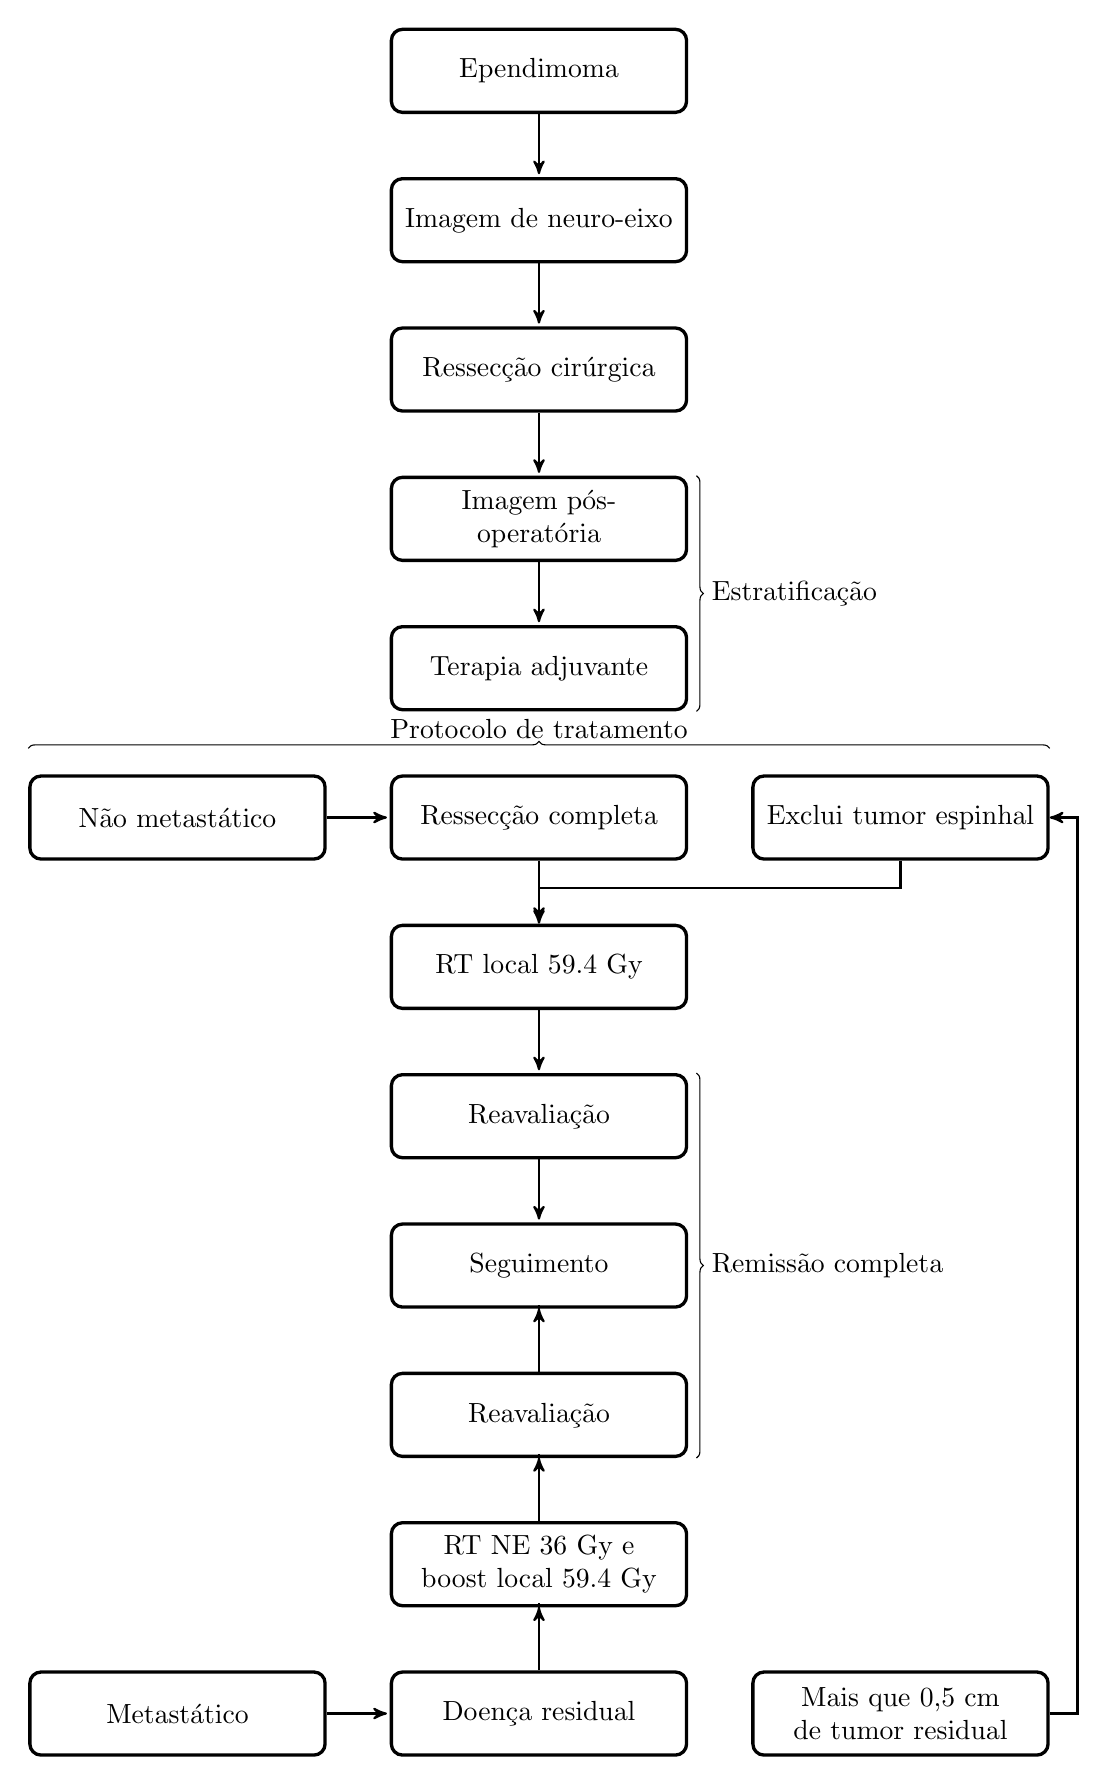
\begin{tikzpicture}
  [node distance=.8cm,
  start chain=going below,]
    \node[punktchain, join] (tc) {Ependimoma};
    \node[punktchain, join] (ine)      {Imagem de neuro-eixo};
    \node[punktchain, join] (rc)      {Ressecção cirúrgica};
    \node[punktchain, join] (ipo) {Imagem pós-operatória};
    \node[punktchain, join] (ta) {Terapia adjuvante};
    \node (rco) [punktchain ]  {Ressecção completa};
    \begin{scope}[start branch=venstre,
        %We need to redefine the join-style to have the -> turn out right
        every join/.style={->, thick, shorten <=1pt}, ]
        \node[punktchain, on chain=going left, join=by {<-}]
            (nme) {Não metastático};
    \end{scope}
    \begin{scope}[start branch=hoejre,]
        \node (excspin) [punktchain, on chain=going right] {Exclui tumor espinhal};
    \end{scope}
    \node[punktchain, join,] (rt) {RT local 59.4 Gy};
    \node[punktchain, join,] (reav) {Reavaliação};
    \node[punktchain, join] (seg) {Seguimento};
    \node[punktchain] (reav2) {Reavaliação};
    \node[punktchain] (rtne) {RT NE 36 Gy e boost local 59.4 Gy};
    \node (dor) [punktchain ]  {Doença residual};
    \begin{scope}[start branch=venstre,
        %We need to redefine the join-style to have the -> turn out right
        every join/.style={->, thick, shorten <=1pt}, ]
        \node[punktchain, on chain=going left, join=by {<-}]
            (me) {Metastático};
    \end{scope}
    \begin{scope}[start branch=hoejre,]
        \node (rci) [punktchain, on chain=going right] 
            {Mais que 0,5 cm de tumor residual};
    \end{scope}
    
  % Now that we have finished the main figure let us add some "after-drawings"
  %% First, let us connect (finans) with (disk). We want it to have
  %% square corners.
  \draw[|-,-|,->, thick,] (excspin.south) |-+(0,-1em)-| (rt.north);
  \draw[-|,|-,->, thick,] (rci.east) -|+(1em,0)|- (excspin.east);
  \draw[-,->, thick,] (dor.north) -|+(0,0)|- (rtne.south);
  \draw[-,->, thick,] (rtne.north) -|+(0,0)|- (reav2.south);
  \draw[-,->, thick,] (reav2.north) -|+(0,0)|- (seg.south);
  % Now, let us add some braches. 
  %% No. 1
  \draw[tuborg] let
    \p1=(nme.west), \p2=(excspin.east) in
    ($(\x1,\y1+2.5em)$) -- ($(\x2,\y2+2.5em)$) node[above, midway]  {Protocolo de tratamento};
  %% No. 2
  \draw[tuborg, decoration={brace}] let \p1=(reav.north), \p2=(reav2.south) in
    ($(2, \y1)$) -- ($(2, \y2)$) node[tubnode] {Remissão completa};
  %% No. 3
  \draw[tuborg, decoration={brace}] let \p1=(ipo.north), \p2=(ta.south) in
    ($(2, \y1)$) -- ($(2, \y2)$) node[tubnode] {Estratificação};
  \end{tikzpicture}

\cleardoublepage

\section{Tumores embrionários -- Adaptado dos ensaios COG-A99701 e ACNS0332}
{\let\thefootnote\relax\footnotetext{Versão Junho/2019}}
\textbf{Racional:} no estudo piloto do COG\cite{jak}, a QT durante a RT possibilitou a melhora da sobrevida de pacientes com tumor residual ou metástase. O COG está testando agora essa estratégia no ensaio fase III ACNS0332. Resultados preliminares para tumores embrionários supratentoriais mostraram que a adição de carboplatina durante a RT não modificou a sobrevida, não podendo ser recomendada para este subgrupo de pacientes.\cite{doi:10.1200/JCO.2017.76.4720}  Não existe tratamento quimioterápico padrão para estes pacientes, porém os resultados do COG são os melhores publicados até o momento. Reforço deve ser feito também sobre as metástases espinhais, até 45Gy dose total acima do cone medular e 50,4 Gy abaixo dele. Reavaliar com imagens 4 semanas após terminar RT.

\textbf{Elegível:} meduloblastoma (fossa posterior) e PNET, com mais de 1,5cm\textsuperscript{2} de tumor residual (RNM de controle até 21 dias pós-op, preferido 72h após); e/ou com metástases (RNM de neuro-eixo e PL/MO); incluir tumores com anaplasia ou positivos para N-MYC/C-MYC. Excluir pacientes com marcador INI-1 negativo ou menores de 3 anos. Tratamento precisa iniciar até 31 dias após cirurgia. NÃO INICIAR ESTE PROTOCOLO EM CRIANÇAS GRAVEMENTE ENFERMAS.

\textbf{Alternativa:} não existe alternativa de QT amplamente aceita para este grupo de pacientes. Invariavelmente, os pacientes com doença metastática e fatores de risco molecular têm prognóstico insatisfatório, com reduzida sobrevida livre de progressão prolongada.
\cleardoublepage
    \noindent
\entrywithlabel[1\hsize]{\textbf{Nome}}\hfill
\\[0.3cm]
\entrywithlabel[.45\hsize]{\textbf{Peso}}\hfill  \entrywithlabel[.45\hsize]{\textbf{Estatura}}

\subsection{Radioquimioterapia: 7 semanas (43 dias)}
Não fazer este componente para pacientes com tumores embrionários supratentoriais. Deve ser feito apenas para pacientes com meduloblastoma de alto risco.

\begin{center}
\begin{table}[H]
\begin{tabular}{p{1cm}p{2cm}|p{2cm}|p{1cm}|p{4cm}|p{3cm}}
	\hline
	\multicolumn{6}{c}{\textbf{SEMANA 1}}\\
\hline
    \multicolumn{1}{c|}{\multirow{2}{*}{\textbf{Dia}}}&\multicolumn{2}{c|}{Dose RT}&\multicolumn{1}{c|}{\multirow{2}{*}{Data}}&\multicolumn{1}{c|}{\multirow{2}{*}{Quimioterapia}}&\multicolumn{1}{c}{\multirow{2}{*}{Rubrica}} \\
    \cline{2-3}
    \multicolumn{1}{c|}{\multirow{1}{*}{}}&{Neuro-eixo}&{Fossa poster}&& \\
	\hline
	\multicolumn{1}{c|}{\multirow{1}{*}{\textbf{D1}}}&\multicolumn{1}{c|}{}&{\(1,8\) Gy}&&{Vincristina \(1,5\) mg/m\(^2\)}&\\
	\multicolumn{1}{c|}{\multirow{1}{*}{\textbf{}}}&\multicolumn{1}{c|}{}&&&{Carboplatina 35mg/m\textsuperscript{2}}&\\
    \multicolumn{1}{c|}{\multirow{1}{*}{\textbf{D2}}}&\multicolumn{1}{c|}{}&{\(1,8\) Gy}&&{Carboplatina 35mg/m\textsuperscript{2}}&\\
    \multicolumn{1}{c|}{\multirow{1}{*}{\textbf{D3}}}&\multicolumn{1}{c|}{}&{\(1,8\) Gy}&&{Carboplatina 35mg/m\textsuperscript{2}}&\\
    \multicolumn{1}{c|}{\multirow{1}{*}{\textbf{D4}}}&\multicolumn{1}{c|}{}&{\(1,8\) Gy}&&{Carboplatina 35mg/m\textsuperscript{2}}&\\
    \multicolumn{1}{c|}{\multirow{1}{*}{\textbf{D5}}}&\multicolumn{1}{c|}{}&{\(1,8\) Gy}&&{Carboplatina 35mg/m\textsuperscript{2}}&\\
    \hline
    \multicolumn{1}{c|}{\multirow{2}{*}{\textbf{Exames}}}&\multicolumn{2}{l|}{Neut (\(>7,5\times10^2\)):}&\multicolumn{2}{l|}{Plaq (\(>7,5\times10^4\)):}&\\
    \cline{2-6}
    \multicolumn{1}{c|}{\multirow{2}{*}{{}}}&\multicolumn{2}{l|}{BT(<1,9mg/dl):}&\multicolumn{2}{l|}{BD(\(<1,5\)mg/dl):}&\\
    \hline
\end{tabular}
\end{table}
\begin{table}[H]
\begin{tabular}{p{1cm}p{2cm}|p{2cm}|p{1cm}|p{4cm}|p{3cm}}
	\hline
	\multicolumn{6}{c}{\textbf{SEMANA 2}}\\
\hline
    \multicolumn{1}{c|}{\multirow{2}{*}{\textbf{Dia}}}&\multicolumn{2}{c|}{Dose RT}&\multicolumn{1}{c|}{\multirow{2}{*}{Data}}&\multicolumn{1}{c|}{\multirow{2}{*}{Quimioterapia}}&\multicolumn{1}{c}{\multirow{2}{*}{Rubrica}} \\
    \cline{2-3}
    \multicolumn{1}{c|}{\multirow{1}{*}{}}&{Neuro-eixo}&{Fossa poster}&& \\
	\hline
	\multicolumn{1}{c|}{\multirow{1}{*}{\textbf{D8}}}&\multicolumn{1}{c|}{}&{\(1,8\) Gy}&&{Vincristina \(1,5\) mg/m\(^2\)}&\\
	\multicolumn{1}{c|}{\multirow{1}{*}{\textbf{}}}&\multicolumn{1}{c|}{}&&&{Carboplatina 35mg/m\textsuperscript{2}}&\\
    \multicolumn{1}{c|}{\multirow{1}{*}{\textbf{D9}}}&\multicolumn{1}{c|}{}&{\(1,8\) Gy}&&{Carboplatina 35mg/m\textsuperscript{2}}&\\
    \multicolumn{1}{c|}{\multirow{1}{*}{\textbf{D10}}}&\multicolumn{1}{c|}{}&{\(1,8\) Gy}&&{Carboplatina 35mg/m\textsuperscript{2}}&\\
    \multicolumn{1}{c|}{\multirow{1}{*}{\textbf{D11}}}&\multicolumn{1}{c|}{}&{\(1,8\) Gy}&&{Carboplatina 35mg/m\textsuperscript{2}}&\\
    \multicolumn{1}{c|}{\multirow{1}{*}{\textbf{D12}}}&\multicolumn{1}{c|}{}&{\(1,8\) Gy}&&{Carboplatina 35mg/m\textsuperscript{2}}&\\
    \hline
    \multicolumn{1}{c|}{\multirow{2}{*}{\textbf{Exames}}}&\multicolumn{2}{l|}{Neut (\(>7,5\times10^2\)):}&\multicolumn{2}{l|}{Plaq (\(>7,5\times10^4\)):}&\\
    \cline{2-6}
    \multicolumn{1}{c|}{\multirow{2}{*}{{}}}&\multicolumn{2}{l|}{BT(<1,9mg/dl):}&\multicolumn{2}{l|}{BD(\(<1,5\)mg/dl):}&\\
    \hline
\end{tabular}
\end{table}
\begin{table}[H]
\begin{tabular}{p{1cm}p{2cm}|p{2cm}|p{1cm}|p{4cm}|p{3cm}}
	\hline
	\multicolumn{6}{c}{\textbf{SEMANA 3}}\\
\hline
    \multicolumn{1}{c|}{\multirow{2}{*}{\textbf{Dia}}}&\multicolumn{2}{c|}{Dose RT}&\multicolumn{1}{c|}{\multirow{2}{*}{Data}}&\multicolumn{1}{c|}{\multirow{2}{*}{Quimioterapia}}&\multicolumn{1}{c}{\multirow{2}{*}{Rubrica}} \\
    \cline{2-3}
    \multicolumn{1}{c|}{\multirow{1}{*}{}}&{Neuro-eixo}&{Fossa poster}&& \\
	\hline
	\multicolumn{1}{c|}{\multirow{1}{*}{\textbf{D15}}}&\multicolumn{1}{c|}{\(1,8\) Gy}&&&{Vincristina \(1,5\) mg/m\(^2\)}&\\
	\multicolumn{1}{c|}{\multirow{1}{*}{\textbf{}}}&\multicolumn{1}{c|}{}&&&{Carboplatina 35mg/m\textsuperscript{2}}&\\
    \multicolumn{1}{c|}{\multirow{1}{*}{\textbf{D16}}}&\multicolumn{1}{c|}{\(1,8\) Gy}&&&{Carboplatina 35mg/m\textsuperscript{2}}&\\
    \multicolumn{1}{c|}{\multirow{1}{*}{\textbf{D17}}}&\multicolumn{1}{c|}{\(1,8\) Gy}&&&{Carboplatina 35mg/m\textsuperscript{2}}&\\
    \multicolumn{1}{c|}{\multirow{1}{*}{\textbf{D18}}}&\multicolumn{1}{c|}{\(1,8\) Gy}&&&{Carboplatina 35mg/m\textsuperscript{2}}&\\
    \multicolumn{1}{c|}{\multirow{1}{*}{\textbf{D19}}}&\multicolumn{1}{c|}{\(1,8\) Gy}&&&{Carboplatina 35mg/m\textsuperscript{2}}&\\
    \hline
    \multicolumn{1}{c|}{\multirow{2}{*}{\textbf{Exames}}}&\multicolumn{2}{l|}{Neut (\(>7,5\times10^2\)):}&\multicolumn{2}{l|}{Plaq (\(>7,5\times10^4\)):}&\\
    \cline{2-6}
    \multicolumn{1}{c|}{\multirow{2}{*}{{}}}&\multicolumn{2}{l|}{BT(<1,9mg/dl):}&\multicolumn{2}{l|}{BD(\(<1,5\)mg/dl):}&
    \\
    \hline
\end{tabular}
\end{table}
\begin{table}[H]
\begin{tabular}{p{1cm}p{2cm}|p{2cm}|p{1cm}|p{4cm}|p{3cm}}
	\hline
	\multicolumn{6}{c}{\textbf{SEMANA 4}}\\
\hline
    \multicolumn{1}{c|}{\multirow{2}{*}{\textbf{Dia}}}&\multicolumn{2}{c|}{Dose RT}&\multicolumn{1}{c|}{\multirow{2}{*}{Data}}&\multicolumn{1}{c|}{\multirow{2}{*}{Quimioterapia}}&\multicolumn{1}{c}{\multirow{2}{*}{Rubrica}} \\
    \cline{2-3}
    \multicolumn{1}{c|}{\multirow{1}{*}{}}&{Neuro-eixo}&{Fossa poster}&& \\
	\hline
	\multicolumn{1}{c|}{\multirow{1}{*}{\textbf{D22}}}&\multicolumn{1}{c|}{\(1,8\) Gy}&&&{Vincristina \(1,5\) mg/m\(^2\)}&\\
	\multicolumn{1}{c|}{\multirow{1}{*}{\textbf{}}}&\multicolumn{1}{c|}{}&&&{Carboplatina 35mg/m\textsuperscript{2}}&\\
    \multicolumn{1}{c|}{\multirow{1}{*}{\textbf{D23}}}&\multicolumn{1}{c|}{\(1,8\) Gy}&&&{Carboplatina 35mg/m\textsuperscript{2}}&\\
    \multicolumn{1}{c|}{\multirow{1}{*}{\textbf{D24}}}&\multicolumn{1}{c|}{\(1,8\) Gy}&&&{Carboplatina 35mg/m\textsuperscript{2}}&\\
    \multicolumn{1}{c|}{\multirow{1}{*}{\textbf{D25}}}&\multicolumn{1}{c|}{\(1,8\) Gy}&&&{Carboplatina 35mg/m\textsuperscript{2}}&\\
    \multicolumn{1}{c|}{\multirow{1}{*}{\textbf{D26}}}&\multicolumn{1}{c|}{\(1,8\) Gy}&&&{Carboplatina 35mg/m\textsuperscript{2}}&\\
    \hline
    \multicolumn{1}{c|}{\multirow{2}{*}{\textbf{Exames}}}&\multicolumn{2}{l|}{Neut (\(>7,5\times10^2\)):}&\multicolumn{2}{l|}{Plaq (\(>7,5\times10^4\)):}&\\
    \cline{2-6}
    \multicolumn{1}{c|}{\multirow{2}{*}{{}}}&\multicolumn{2}{l|}{BT(<1,9mg/dl):}&\multicolumn{2}{l|}{BD(\(<1,5\)mg/dl):}&
    \\
    \hline
\end{tabular}
\end{table}

\begin{table}[H]
\begin{tabular}{p{1cm}p{2cm}|p{2cm}|p{1cm}|p{4cm}|p{3cm}}
	\hline
	\multicolumn{6}{c}{\textbf{SEMANA 5}}\\
\hline
    \multicolumn{1}{c|}{\multirow{2}{*}{\textbf{Dia}}}&\multicolumn{2}{c|}{Dose RT}&\multicolumn{1}{c|}{\multirow{2}{*}{Data}}&\multicolumn{1}{c|}{\multirow{2}{*}{Quimioterapia}}&\multicolumn{1}{c}{\multirow{2}{*}{Rubrica}} \\
    \cline{2-3}
    \multicolumn{1}{c|}{\multirow{1}{*}{}}&{Neuro-eixo}&{Fossa poster}&& \\
	\hline
	\multicolumn{1}{c|}{\multirow{1}{*}{\textbf{D29}}}&\multicolumn{1}{c|}{\(1,8\) Gy}&&&{Vincristina \(1,5\) mg/m\(^2\)}&\\
	\multicolumn{1}{c|}{\multirow{1}{*}{\textbf{}}}&\multicolumn{1}{c|}{}&&&{Carboplatina 35mg/m\textsuperscript{2}}&\\
    \multicolumn{1}{c|}{\multirow{1}{*}{\textbf{D30}}}&\multicolumn{1}{c|}{\(1,8\) Gy}&&&{Carboplatina 35mg/m\textsuperscript{2}}&\\
    \multicolumn{1}{c|}{\multirow{1}{*}{\textbf{D31}}}&\multicolumn{1}{c|}{\(1,8\) Gy}&&&{Carboplatina 35mg/m\textsuperscript{2}}&\\
    \multicolumn{1}{c|}{\multirow{1}{*}{\textbf{D32}}}&\multicolumn{1}{c|}{\(1,8\) Gy}&&&{Carboplatina 35mg/m\textsuperscript{2}}&\\
    \multicolumn{1}{c|}{\multirow{1}{*}{\textbf{D33}}}&\multicolumn{1}{c|}{\(1,8\) Gy}&&&{Carboplatina 35mg/m\textsuperscript{2}}&\\
    \hline
    \multicolumn{1}{c|}{\multirow{2}{*}{\textbf{Exames}}}&\multicolumn{2}{l|}{Neut (\(>7,5\times10^2\)):}&\multicolumn{2}{l|}{Plaq (\(>7,5\times10^4\)):}&\\
    \cline{2-6}
    \multicolumn{1}{c|}{\multirow{2}{*}{{}}}&\multicolumn{2}{l|}{BT(<1,9mg/dl):}&\multicolumn{2}{l|}{BD(\(<1,5\)mg/dl):}&
    \\
    \hline
\end{tabular}
\end{table}
\begin{table}[H]
\begin{tabular}{p{1cm}p{2cm}|p{2cm}|p{1cm}|p{4cm}|p{3cm}}
	\hline
	\multicolumn{6}{c}{\textbf{SEMANA 6}}\\
\hline
    \multicolumn{1}{c|}{\multirow{2}{*}{\textbf{Dia}}}&\multicolumn{2}{c|}{Dose RT}&\multicolumn{1}{c|}{\multirow{2}{*}{Data}}&\multicolumn{1}{c|}{\multirow{2}{*}{Quimioterapia}}&\multicolumn{1}{c}{\multirow{2}{*}{Rubrica}} \\
    \cline{2-3}
    \multicolumn{1}{c|}{\multirow{1}{*}{}}&{Neuro-eixo}&{Fossa poster}&& \\
	\hline
	\multicolumn{1}{c|}{\multirow{1}{*}{\textbf{D36}}}&\multicolumn{1}{c|}{\(1,8\) Gy}&&&{Vincristina \(1,5\) mg/m\(^2\)}&\\
	\multicolumn{1}{c|}{\multirow{1}{*}{\textbf{}}}&\multicolumn{1}{c|}{}&&&{Carboplatina 35mg/m\textsuperscript{2}}&\\
    \multicolumn{1}{c|}{\multirow{1}{*}{\textbf{D37}}}&\multicolumn{1}{c|}{\(1,8\) Gy}&&&{Carboplatina 35mg/m\textsuperscript{2}}&\\
    \multicolumn{1}{c|}{\multirow{1}{*}{\textbf{D38}}}&\multicolumn{1}{c|}{\(1,8\) Gy}&&&{Carboplatina 35mg/m\textsuperscript{2}}&\\
    \multicolumn{1}{c|}{\multirow{1}{*}{\textbf{D39}}}&\multicolumn{1}{c|}{\(1,8\) Gy}&&&{Carboplatina 35mg/m\textsuperscript{2}}&\\
    \multicolumn{1}{c|}{\multirow{1}{*}{\textbf{D40}}}&\multicolumn{1}{c|}{\(1,8\) Gy}&&&{Carboplatina 35mg/m\textsuperscript{2}}&\\
    \hline
    \multicolumn{1}{c|}{\multirow{2}{*}{\textbf{Exames}}}&\multicolumn{2}{l|}{Neut (\(>7,5\times10^2\)):}&\multicolumn{2}{l|}{Plaq (\(>7,5\times10^4\)):}&\\
    \cline{2-6}
    \multicolumn{1}{c|}{\multirow{2}{*}{{}}}&\multicolumn{2}{l|}{BT(<1,9mg/dl):}&\multicolumn{2}{l|}{BD(\(<1,5\)mg/dl):}&
    \\
    \hline
\end{tabular}
\end{table}
\begin{table}[H]
\begin{tabular}{p{1cm}p{2cm}|p{2cm}|p{1cm}|p{4cm}|p{3cm}}
	\hline
	\multicolumn{6}{c}{\textbf{SEMANA 7}}\\
\hline
    \multicolumn{1}{c|}{\multirow{2}{*}{\textbf{Dia}}}&\multicolumn{2}{c|}{Dose RT}&\multicolumn{1}{c|}{\multirow{2}{*}{Data}}&\multicolumn{1}{c|}{\multirow{2}{*}{Quimioterapia}}&\multicolumn{1}{c}{\multirow{2}{*}{Rubrica}} \\
    \cline{2-3}
    \multicolumn{1}{c|}{\multirow{1}{*}{}}&{Neuro-eixo}&{Fossa poster}&& \\
	\hline
	\multicolumn{1}{c|}{\multirow{1}{*}{\textbf{D43}}}&\multicolumn{1}{c|}{\(1,8\) Gy}&&&{Vincristina \(1,5\) mg/m\(^2\)}&\\
    \hline
    \multicolumn{1}{c|}{\multirow{2}{*}{\textbf{Exames}}}&\multicolumn{2}{l|}{Neut (\(>7,5\times10^2\)):}&\multicolumn{2}{l|}{Plaq (\(>7,5\times10^4\)):}&\\
    \cline{2-6}
    \multicolumn{1}{c|}{\multirow{2}{*}{{}}}&\multicolumn{2}{l|}{BT(<1,9mg/dl):}&\multicolumn{2}{l|}{BD(\(<1,5\)mg/dl):}&
    \\
    \hline
\end{tabular}
\end{table}
\textbf{Intervalo de 42 dias}\\
\end{center}

\pagebreak
    \noindent
\entrywithlabel[1\hsize]{\textbf{Nome}}\hfill
\\[0.3cm]
\entrywithlabel[.45\hsize]{\textbf{Peso}}\hfill  \entrywithlabel[.45\hsize]{\textbf{Estatura}}

\subsection{Manutenção: 06 ciclos}

\begin{center}
\begin{table}[H]
    \begin{tabular}{p{1cm}p{6cm}|p{1cm}|p{3cm}|p{2.5cm}}
    \hline
	\multicolumn{5}{c}{\textbf{CICLO 1}}\\
	\hline
    \multicolumn{1}{c|}{\multirow{1}{*}{\textbf{Dia}}}&{Dose}&{Data}&{Administrado}&{Rubrica} \\
    \hline
    \multicolumn{1}{c|}{\multirow{1}{*}{\textbf{D85}}}&{Ciclofosfamida \(1,0\) g/m\(^2\) EV em 6h}&&{(  ) Sim (  ) Não}&\\
    \multicolumn{1}{c|}{\multirow{1}{*}{\textbf{D86}}}&{Ciclofosfamida \(1,0\) g/m\(^2\) EV em 6h}&&{(  ) Sim (  ) Não}&\\
    \multicolumn{1}{c|}{\multirow{1}{*}{\textbf{}}}&{Vincristina \(1,5\) mg/m\(^2\), max \(2\) mg}&&{(  ) Sim (  ) Não}&\\
    \hline
    \multicolumn{1}{c|}{\multirow{2}{*}{\textbf{Exames}}}&\multicolumn{2}{l|}{Neut(\(>10^3\)):}&{Plaq(\(>10^5\)):}&\\
    \cline{2-5}
    \multicolumn{1}{c|}{\multirow{2}{*}{{}}}&\multicolumn{2}{l|}{ClearCreat (\(>75\%\)) basal:}&{}&{}\\
    \hline
    \\
    \hline
    \multicolumn{1}{c|}{\multirow{1}{*}{\textbf{D92}}}&{Vincristina \(1,5\) mg/m\(^2\), max \(2\) mg}&&{(  ) Sim (  ) Não}&\\
    \hline
\end{tabular}
\end{table}
\textbf{Intervalo de 21 dias}
\begin{table}[H]
\begin{tabular}{p{1cm}p{6cm}|p{1cm}|p{3cm}|p{2.5cm}}
    \hline
	\multicolumn{5}{c}{\textbf{CICLO 2}}\\
	\hline
    \multicolumn{1}{c|}{\multirow{1}{*}{\textbf{Dia}}}&{Dose}&{Data}&{Administrado}&{Rubrica} \\
    \hline
    \multicolumn{1}{c|}{\multirow{1}{*}{\textbf{D113}}}&{Ciclofosfamida \(1,0\) g/m\(^2\) EV em 6h}&&{(  ) Sim (  ) Não}&\\
    \multicolumn{1}{c|}{\multirow{1}{*}{\textbf{D114}}}&{Ciclofosfamida \(1,0\) g/m\(^2\) EV em 6h}&&{(  ) Sim (  ) Não}&\\
    \multicolumn{1}{c|}{\multirow{1}{*}{\textbf{}}}&{Vincristina \(1,5\) mg/m\(^2\), max \(2\) mg}&&{(  ) Sim (  ) Não}&\\
    \hline
    \multicolumn{1}{c|}{\multirow{2}{*}{\textbf{Exames}}}&\multicolumn{2}{l|}{Neut(\(>10^3\)):}&{Plaq(\(>10^5\)):}&\\
    \cline{2-5}
    \multicolumn{1}{c|}{\multirow{2}{*}{{}}}&\multicolumn{2}{l|}{ClearCreat (\(>75\%\)) basal:}&{}&{}\\
    \hline
    \\
    \hline
    \multicolumn{1}{c|}{\multirow{1}{*}{\textbf{D120}}}&{Vincristina \(1,5\) mg/m\(^2\), max \(2\) mg}&&{(  ) Sim (  ) Não}&\\
    \hline
\end{tabular}
\end{table}
\textbf{Intervalo de 21 dias}

\begin{table}[H]
\begin{tabular}{p{1cm}p{6cm}|p{1cm}|p{3cm}|p{2.5cm}}
    \hline
	\multicolumn{5}{c}{\textbf{CICLO 3}}\\
	\hline
    \multicolumn{1}{c|}{\multirow{1}{*}{\textbf{Dia}}}&{Dose}&{Data}&{Administrado}&{Rubrica} \\
    \hline
    \multicolumn{1}{c|}{\multirow{1}{*}{\textbf{D141}}}&{Ciclofosfamida \(1,0\) g/m\(^2\) EV em 6h}&&{(  ) Sim (  ) Não}&\\
    \multicolumn{1}{c|}{\multirow{1}{*}{\textbf{D142}}}&{Ciclofosfamida \(1,0\) g/m\(^2\) EV em 6h}&&{(  ) Sim (  ) Não}&\\
    \multicolumn{1}{c|}{\multirow{1}{*}{\textbf{}}}&{Vincristina \(1,5\) mg/m\(^2\), max \(2\) mg}&&{(  ) Sim (  ) Não}&\\
    \hline
    \multicolumn{1}{c|}{\multirow{2}{*}{\textbf{Exames}}}&\multicolumn{2}{l|}{Neut(\(>10^3\)):}&{Plaq(\(>10^5\)):}&\\
    \cline{2-5}
    \multicolumn{1}{c|}{\multirow{2}{*}{{}}}&\multicolumn{2}{l|}{ClearCreat (\(>75\%\)) basal:}&{}&{}\\
    \hline
    \\
    \hline
    \multicolumn{1}{c|}{\multirow{1}{*}{\textbf{D148}}}&{Vincristina \(1,5\) mg/m\(^2\), max \(2\) mg}&&{(  ) Sim (  ) Não}&\\
    \hline
\end{tabular}
\end{table}
\textbf{Intervalo de 21 dias}

\begin{table}[H]
\begin{tabular}{p{1cm}p{6cm}|p{1cm}|p{3cm}|p{2.5cm}}
    \hline
	\multicolumn{5}{c}{\textbf{CICLO 4}}\\
	\hline
    \multicolumn{1}{c|}{\multirow{1}{*}{\textbf{Dia}}}&{Dose}&{Data}&{Administrado}&{Rubrica} \\
    \hline
    \multicolumn{1}{c|}{\multirow{1}{*}{\textbf{D169}}}&{Ciclofosfamida \(1,0\) g/m\(^2\) EV em 6h}&&{(  ) Sim (  ) Não}&\\
    \multicolumn{1}{c|}{\multirow{1}{*}{\textbf{D170}}}&{Ciclofosfamida \(1,0\) g/m\(^2\) EV em 6h}&&{(  ) Sim (  ) Não}&\\
    \multicolumn{1}{c|}{\multirow{1}{*}{\textbf{}}}&{Vincristina \(1,5\) mg/m\(^2\), max \(2\) mg}&&{(  ) Sim (  ) Não}&\\
    \hline
    \multicolumn{1}{c|}{\multirow{2}{*}{\textbf{Exames}}}&\multicolumn{2}{l|}{Neut(\(>10^3\)):}&{Plaq(\(>10^5\)):}&\\
    \cline{2-5}
    \multicolumn{1}{c|}{\multirow{2}{*}{{}}}&\multicolumn{2}{l|}{ClearCreat (\(>75\%\)) basal:}&{}&{}\\
    \hline\\
    \hline
    \multicolumn{1}{c|}{\multirow{1}{*}{\textbf{D176}}}&{Vincristina \(1,5\) mg/m\(^2\), max \(2\) mg}&&{(  ) Sim (  ) Não}&\\
    \hline
\end{tabular}
\end{table}
\textbf{Intervalo de 21 dias}
\begin{table}[H]
\begin{tabular}{p{1cm}p{6cm}|p{1cm}|p{3cm}|p{2.5cm}}
    \hline
	\multicolumn{5}{c}{\textbf{CICLO 5}}\\
	\hline
    \multicolumn{1}{c|}{\multirow{1}{*}{\textbf{Dia}}}&{Dose}&{Data}&{Administrado}&{Rubrica} \\
    \hline
    \multicolumn{1}{c|}{\multirow{1}{*}{\textbf{D197}}}&{Ciclofosfamida \(1,0\) g/m\(^2\) EV em 6h}&&{(  ) Sim (  ) Não}&\\
    \multicolumn{1}{c|}{\multirow{1}{*}{\textbf{D198}}}&{Ciclofosfamida \(1,0\) g/m\(^2\) EV em 6h}&&{(  ) Sim (  ) Não}&\\
    \multicolumn{1}{c|}{\multirow{1}{*}{\textbf{}}}&{Vincristina \(1,5\) mg/m\(^2\), max \(2\) mg}&&{(  ) Sim (  ) Não}&\\
    \hline
    \multicolumn{1}{c|}{\multirow{2}{*}{\textbf{Exames}}}&\multicolumn{2}{l|}{Neut(\(>10^3\)):}&{Plaq(\(>10^5\)):}&\\
    \cline{2-5}
    \multicolumn{1}{c|}{\multirow{2}{*}{{}}}&\multicolumn{2}{l|}{ClearCreat (\(>75\%\)) basal:}&{}&{}\\
    \hline
    \\
    \hline
    \multicolumn{1}{c|}{\multirow{1}{*}{\textbf{D204}}}&{Vincristina \(1,5\) mg/m\(^2\), max \(2\) mg}&&{(  ) Sim (  ) Não}&\\
    \hline
\end{tabular}
\end{table}
\textbf{Intervalo de 21 dias}
\begin{table}[H]
\begin{tabular}{p{1cm}p{6cm}|p{1cm}|p{3cm}|p{2.5cm}}
    \hline
	\multicolumn{5}{c}{\textbf{CICLO 6}}\\
	\hline
    \multicolumn{1}{c|}{\multirow{1}{*}{\textbf{Dia}}}&{Dose}&{Data}&{Administrado}&{Rubrica} \\
    \hline
    \multicolumn{1}{c|}{\multirow{1}{*}{\textbf{D225}}}&{Ciclofosfamida \(1,0\) g/m\(^2\) EV em 6h}&&{(  ) Sim (  ) Não}&\\
    \multicolumn{1}{c|}{\multirow{1}{*}{\textbf{D226}}}&{Ciclofosfamida \(1,0\) g/m\(^2\) EV em 6h}&&{(  ) Sim (  ) Não}&\\
    \multicolumn{1}{c|}{\multirow{1}{*}{\textbf{}}}&{Vincristina \(1,5\) mg/m\(^2\), max \(2\) mg}&&{(  ) Sim (  ) Não}&\\
    \hline
    \multicolumn{1}{c|}{\multirow{2}{*}{\textbf{Exames}}}&\multicolumn{2}{l|}{Neut(\(>10^3\)):}&{Plaq(\(>10^5\)):}&\\
    \cline{2-5}
    \multicolumn{1}{c|}{\multirow{2}{*}{{}}}&\multicolumn{2}{l|}{ClearCreat (\(>75\%\)):}&{}&{}\\
    \hline
    \\
    \hline
    \multicolumn{1}{c|}{\multirow{1}{*}{\textbf{D232}}}&{Vincristina \(1,5\) mg/m\(^2\), max \(2\) mg}&&{(  ) Sim (  ) Não}&\\
    \hline
\end{tabular}
\end{table}
\textbf{FIM DE PROTOCOLO}

\end{center}
\subsection{Modificações de dose:}
Se tiver que adiar a CTX por neutropenia, reduzir em 25\% a dose, mesmo após recuperação.Toxicidade grau 3-4 pela VCR, suspender dose seguinte. Reiniciar com dose normal. Recorrência: reduzir dose.

\textbf{Avaliação:} imagem a cada 3 ciclos (3 meses), se progressão, interromper protocolo.

\textbf{ATENÇÃO:} este protocolo mostrou eficácia em um ensaio fase II não comparativo com número limitado de pacientes. Dessa forma, é inadequado iniciar este protocolo em crianças com risco de complicações graves, como naquelas que têm sequelas importantes e muito limitantes.

\cleardoublepage

\section{Glioma de alto grau -- Adaptado do ensaio ACNS0423}
{\let\thefootnote\relax\footnotetext{Versão Junho/2019}}
\textbf{Racional:} no estudo do COG, a temozolomida (TMZ) associada à lomustina mostraram superioridade em relação ao controle histórico (ACNS0126)\cite{10.1093/neuonc/now038}. Deve-se levar em conta a disponibilidade e custo do esquema. Não foi realizada comparação com os dados do estudo CCG-945.

\textbf{Elegível:} extensão da ressecção cirúrgica (RNM de controle até 21 dias pós-op, preferido 72h após); não é necessário pesquisar metástases de rotina (RNM de neuro-eixo e PL/MO). Tratamento precisa iniciar até 42 dias após cirurgia. Inclui glioblastoma multiforme, astrocitoma anaplásico, oligodendroglioma anaplásico, gliossarcoma. Pacientes com gliomas difusos de linha média H3K27M+ (DIPG) não foram incluídos neste protocolo, porém mostraram ausência de resposta a temozolomida durante e após a radioterapia\cite{10.1093/neuonc/noq205}, logo não devem ser incluídos neste protcolo. Pacientes com mais de 3 anos de idade. Somente iniciar o protocolo após a assinatura do TERMO DE CONSENTIMENTO INFORMADO, conforme acordado. NÃO INICIAR ESTE PROTOCOLO EM CRIANÇAS GRAVEMENTE ENFERMAS.

\textbf{Alternativa:} não existe esquema de QT amplamente aceito para tratar crianças com gliomas de alto grau, incluindo gliomas pontinos intrínsecos difusos (DIPG). O tratamento padrão é RT craniana. Os pacientes com mais de 3 anos têm um prognóstico insatisfatório e sobrevida mediana de pouco mais de 12 meses.
\cleardoublepage

    \noindent
\entrywithlabel[1\hsize]{\textbf{Nome}}\hfill
\\[0.3cm]
\entrywithlabel[.45\hsize]{\textbf{Peso}}\hfill  \entrywithlabel[.45\hsize]{\textbf{Estatura}}

\subsection{Indução: 6 semanas (radioquimioterapia)}

\renewcommand{\arraystretch}{1.5}

\begin{center}
\begin{table}[H]
\begin{tabular}{p{1cm}c|c|c|c|c|c}
	\hline
\multicolumn{1}{c|}{\multirow{1}{*}{\textbf{Semana}}}&{Dose}&{Data}&{Neut}&{Plaq}&{Administrado}&{Rubrica} \\
    \hline
    \multicolumn{1}{c|}{\multirow{1}{*}{\textbf{1}}}&{Temozolomida 90mg/m\textsuperscript{2}/dia Seg-Sex}&{}&&&{(  ) Sim (  ) Não}&\\
    \cline{3-5}
    \multicolumn{1}{c|}{\multirow{1}{*}{{\textbf{2}}}}&{Temozolomida 90mg/m\textsuperscript{2}/dia Seg-Sex}&{}&&&{(  ) Sim (  ) Não}&\\
    \cline{3-5}
    \multicolumn{1}{c|}{\multirow{1}{*}{{\textbf{3}}}}&{Temozolomida 90mg/m\textsuperscript{2}/dia Seg-Sex}&{}&&&{(  ) Sim (  ) Não}&\\
    \cline{3-5}
    \multicolumn{1}{c|}{\multirow{1}{*}{{\textbf{4}}}}&{Temozolomida 90mg/m\textsuperscript{2}/dia Seg-Sex}&{}&&&{(  ) Sim (  ) Não}&\\
    \cline{3-5}
    \multicolumn{1}{c|}{\multirow{1}{*}{{\textbf{5}}}}&{Temozolomida 90mg/m\textsuperscript{2}/dia Seg-Sex}&{}&&&{(  ) Sim (  ) Não}&\\
    \cline{3-5}
    \multicolumn{1}{c|}{\multirow{1}{*}{{\textbf{6}}}}&{Temozolomida 90mg/m\textsuperscript{2}/dia Seg-Sex}&{}&&&{(  ) Sim (  ) Não}&\\
    \hline
\end{tabular}
\end{table}
\textbf{Intervalo de 28 dias.}
\end{center}
\subsection{Manutenção: 06 ciclos}

\begin{center}
\begin{table}[H]
\begin{tabular}{p{1cm}p{5cm}|p{1cm}|p{4.5cm}|p{2cm}}
	\hline
	\multicolumn{5}{c}{\textbf{CICLO 1}}\\
\hline
    \multicolumn{1}{c|}{\multirow{1}{*}{\textbf{Dia}}}&{Dose}&{Data}&{Administrado}&{Rubrica} \\
    \hline
    \multicolumn{1}{c|}{\multirow{1}{*}{\textbf{D1}}}&{Temozolomida \(160\) mg/m\(^2\)}&&{(  ) Sim (  ) Não}&\\
    \multicolumn{1}{c|}{\multirow{1}{*}{\textbf{}}}&{Lomustina \(90\) mg/m\(^2\)}&&{(  ) Sim (  ) Não}&\\
    \multicolumn{1}{c|}{\multirow{1}{*}{\textbf{D2}}}&{Temozolomida \(160\) mg/m\(^2\)}&&{(  ) Sim (  ) Não}&\\
    \multicolumn{1}{c|}{\multirow{1}{*}{\textbf{D3}}}&{Temozolomida \(160\) mg/m\(^2\)}&&{(  ) Sim (  ) Não}&\\
    \multicolumn{1}{c|}{\multirow{1}{*}{\textbf{D4}}}&{Temozolomida \(160\) mg/m\(^2\)}&&{(  ) Sim (  ) Não}&\\
    \multicolumn{1}{c|}{\multirow{1}{*}{\textbf{D5}}}&{Temozolomida \(160\) mg/m\(^2\)}&&{(  ) Sim (  ) Não}&\\
    \hline
    \multicolumn{1}{c|}{\multirow{2}{*}{\textbf{Exames}}}&\multicolumn{2}{l|}{Neut (\(>7,5\times10^2\)):}&{Plaq (\(>7,5\times10^4\)):}&{TGO:}\\
    \cline{2-5}
    \multicolumn{1}{c|}{\multirow{2}{*}{{}}}&\multicolumn{2}{l|}{Creat(\(<1,5\) vezes)}&{BT(\(<1,5\) vezes):}&{TGP:}
    \\
    \hline
\end{tabular}
\end{table}
\textbf{Intervalo de 14 dias.}
\begin{table}[H]
\begin{tabular}{p{5cm}|p{5cm}|p{4.7cm}}
    \hline
    \textbf{Exames (data):}&{Neut (\(>7,5\times10^2\)):}&{Plaq (\(>7,5\times10^4\)):}
    \\
    \hline
\end{tabular}
\end{table}
\textbf{Intervalo de 28 dias.}
\begin{table}[H]
\begin{tabular}{p{1cm}p{5cm}|p{1cm}|p{4.5cm}|p{2cm}}
	\hline
	\multicolumn{5}{c}{\textbf{CICLO 2}}\\
\hline
    \multicolumn{1}{c|}{\multirow{1}{*}{\textbf{Dia}}}&{Dose}&{Data}&{Administrado}&{Rubrica} \\
    \hline
    \multicolumn{1}{c|}{\multirow{1}{*}{\textbf{D1}}}&{Temozolomida \(160\) mg/m\(^2\)}&&{(  ) Sim (  ) Não}&\\
    \multicolumn{1}{c|}{\multirow{1}{*}{\textbf{}}}&{Lomustina \(90\) mg/m\(^2\)}&&{(  ) Sim (  ) Não}&\\
    \multicolumn{1}{c|}{\multirow{1}{*}{\textbf{D2}}}&{Temozolomida \(160\) mg/m\(^2\)}&&{(  ) Sim (  ) Não}&\\
    \multicolumn{1}{c|}{\multirow{1}{*}{\textbf{D3}}}&{Temozolomida \(160\) mg/m\(^2\)}&&{(  ) Sim (  ) Não}&\\
    \multicolumn{1}{c|}{\multirow{1}{*}{\textbf{D4}}}&{Temozolomida \(160\) mg/m\(^2\)}&&{(  ) Sim (  ) Não}&\\
    \multicolumn{1}{c|}{\multirow{1}{*}{\textbf{D5}}}&{Temozolomida \(160\) mg/m\(^2\)}&&{(  ) Sim (  ) Não}&\\
    \hline
    \multicolumn{1}{c|}{\multirow{2}{*}{\textbf{Exames}}}&\multicolumn{2}{l|}{Neut (\(>7,5\times10^2\)):}&{Plaq (\(>7,5\times10^4\)):}&{TGO:}\\
    \cline{2-5}
    \multicolumn{1}{c|}{\multirow{2}{*}{{}}}&\multicolumn{2}{l|}{Creat(\(<1,5\) vezes)}&{BT(\(<1,5\) vezes):}&{TGP:}
    \\
    \hline
\end{tabular}
\end{table}
\textbf{Intervalo de 14 dias.}
\begin{table}[H]
\begin{tabular}{p{5cm}|p{5cm}|p{4.7cm}}
    \hline
    \textbf{Exames (data):}&{Neut (\(>7,5\times10^2\)):}&{Plaq (\(>7,5\times10^4\)):}
    \\
    \hline
\end{tabular}
\end{table}
\textbf{Intervalo de 28 dias.}

\begin{table}[H]
\begin{tabular}{p{1cm}p{5cm}|p{1cm}|p{4.5cm}|p{2cm}}
	\hline
	\multicolumn{5}{c}{\textbf{CICLO 3}}\\
\hline
    \multicolumn{1}{c|}{\multirow{1}{*}{\textbf{Dia}}}&{Dose}&{Data}&{Administrado}&{Rubrica} \\
    \hline
    \multicolumn{1}{c|}{\multirow{1}{*}{\textbf{D1}}}&{Temozolomida \(160\) mg/m\(^2\)}&&{(  ) Sim (  ) Não}&\\
    \multicolumn{1}{c|}{\multirow{1}{*}{\textbf{}}}&{Lomustina \(90\) mg/m\(^2\)}&&{(  ) Sim (  ) Não}&\\
    \multicolumn{1}{c|}{\multirow{1}{*}{\textbf{D2}}}&{Temozolomida \(160\) mg/m\(^2\)}&&{(  ) Sim (  ) Não}&\\
    \multicolumn{1}{c|}{\multirow{1}{*}{\textbf{D3}}}&{Temozolomida \(160\) mg/m\(^2\)}&&{(  ) Sim (  ) Não}&\\
    \multicolumn{1}{c|}{\multirow{1}{*}{\textbf{D4}}}&{Temozolomida \(160\) mg/m\(^2\)}&&{(  ) Sim (  ) Não}&\\
    \multicolumn{1}{c|}{\multirow{1}{*}{\textbf{D5}}}&{Temozolomida \(160\) mg/m\(^2\)}&&{(  ) Sim (  ) Não}&\\
    \hline
    \multicolumn{1}{c|}{\multirow{2}{*}{\textbf{Exames}}}&\multicolumn{2}{l|}{Neut (\(>7,5\times10^2\)):}&{Plaq (\(>7,5\times10^4\)):}&{TGO:}\\
    \cline{2-5}
    \multicolumn{1}{c|}{\multirow{2}{*}{{}}}&\multicolumn{2}{l|}{Creat(\(<1,5\) vezes)}&{BT(\(<1,5\) vezes):}&{TGP:}
    \\
    \hline
\end{tabular}
\end{table}
\textbf{Intervalo de 14 dias.}
\begin{table}[H]
\begin{tabular}{p{5cm}|p{5cm}|p{4.7cm}}
    \hline
    \textbf{Exames (data):}&{Neut (\(>7,5\times10^2\)):}&{Plaq (\(>7,5\times10^4\)):}
    \\
    \hline
\end{tabular}
\end{table}
\textbf{Intervalo de 28 dias.}

\pagebreak
    \noindent
\entrywithlabel[1\hsize]{\textbf{Nome}}\hfill
\\[0.3cm]
\entrywithlabel[.45\hsize]{\textbf{Peso}}\hfill  \entrywithlabel[.45\hsize]{\textbf{Estatura}}

\begin{table}[H]
\begin{tabular}{p{1cm}p{5cm}|p{1cm}|p{4.5cm}|p{2cm}}
	\hline
	\multicolumn{5}{c}{\textbf{CICLO 4}}\\
\hline
    \multicolumn{1}{c|}{\multirow{1}{*}{\textbf{Dia}}}&{Dose}&{Data}&{Administrado}&{Rubrica} \\
    \hline
    \multicolumn{1}{c|}{\multirow{1}{*}{\textbf{D1}}}&{Temozolomida \(160\) mg/m\(^2\)}&&{(  ) Sim (  ) Não}&\\
    \multicolumn{1}{c|}{\multirow{1}{*}{\textbf{}}}&{Lomustina \(90\) mg/m\(^2\)}&&{(  ) Sim (  ) Não}&\\
    \multicolumn{1}{c|}{\multirow{1}{*}{\textbf{D2}}}&{Temozolomida \(160\) mg/m\(^2\)}&&{(  ) Sim (  ) Não}&\\
    \multicolumn{1}{c|}{\multirow{1}{*}{\textbf{D3}}}&{Temozolomida \(160\) mg/m\(^2\)}&&{(  ) Sim (  ) Não}&\\
    \multicolumn{1}{c|}{\multirow{1}{*}{\textbf{D4}}}&{Temozolomida \(160\) mg/m\(^2\)}&&{(  ) Sim (  ) Não}&\\
    \multicolumn{1}{c|}{\multirow{1}{*}{\textbf{D5}}}&{Temozolomida \(160\) mg/m\(^2\)}&&{(  ) Sim (  ) Não}&\\
    \hline
    \multicolumn{1}{c|}{\multirow{2}{*}{\textbf{Exames}}}&\multicolumn{2}{l|}{Neut (\(>7,5\times10^2\)):}&{Plaq (\(>7,5\times10^4\)):}&{TGO:}\\
    \cline{2-5}
    \multicolumn{1}{c|}{\multirow{2}{*}{{}}}&\multicolumn{2}{l|}{Creat(\(<1,5\) vezes)}&{BT(\(<1,5\) vezes):}&{TGP:}
    \\
    \hline
\end{tabular}
\end{table}
\textbf{Intervalo de 14 dias.}
\begin{table}[H]
\begin{tabular}{p{5cm}|p{5cm}|p{4.7cm}}
    \hline
    \textbf{Exames (data):}&{Neut (\(>7,5\times10^2\)):}&{Plaq (\(>7,5\times10^4\)):}
    \\
    \hline
\end{tabular}
\end{table}
\textbf{Intervalo de 28 dias.}
\begin{table}[H]
\begin{tabular}{p{1cm}p{5cm}|p{1cm}|p{4.5cm}|p{2cm}}
	\hline
	\multicolumn{5}{c}{\textbf{CICLO 5}}\\
\hline
    \multicolumn{1}{c|}{\multirow{1}{*}{\textbf{Dia}}}&{Dose}&{Data}&{Administrado}&{Rubrica} \\
    \hline
    \multicolumn{1}{c|}{\multirow{1}{*}{\textbf{D1}}}&{Temozolomida \(160\) mg/m\(^2\)}&&{(  ) Sim (  ) Não}&\\
    \multicolumn{1}{c|}{\multirow{1}{*}{\textbf{}}}&{Lomustina \(90\) mg/m\(^2\)}&&{(  ) Sim (  ) Não}&\\
    \multicolumn{1}{c|}{\multirow{1}{*}{\textbf{D2}}}&{Temozolomida \(160\) mg/m\(^2\)}&&{(  ) Sim (  ) Não}&\\
    \multicolumn{1}{c|}{\multirow{1}{*}{\textbf{D3}}}&{Temozolomida \(160\) mg/m\(^2\)}&&{(  ) Sim (  ) Não}&\\
    \multicolumn{1}{c|}{\multirow{1}{*}{\textbf{D4}}}&{Temozolomida \(160\) mg/m\(^2\)}&&{(  ) Sim (  ) Não}&\\
    \multicolumn{1}{c|}{\multirow{1}{*}{\textbf{D5}}}&{Temozolomida \(160\) mg/m\(^2\)}&&{(  ) Sim (  ) Não}&\\
    \hline
    \multicolumn{1}{c|}{\multirow{2}{*}{\textbf{Exames}}}&\multicolumn{2}{l|}{Neut (\(>7,5\times10^2\)):}&{Plaq (\(>7,5\times10^4\)):}&{TGO:}\\
    \cline{2-5}
    \multicolumn{1}{c|}{\multirow{2}{*}{{}}}&\multicolumn{2}{l|}{Creat(\(<1,5\) vezes)}&{BT(\(<1,5\) vezes):}&{TGP:}
    \\
    \hline
\end{tabular}
\end{table}
\textbf{Intervalo de 14 dias.}
\begin{table}[H]
\begin{tabular}{p{5cm}|p{5cm}|p{4.7cm}}
    \hline
    \textbf{Exames (data):}&{Neut (\(>7,5\times10^2\)):}&{Plaq (\(>7,5\times10^4\)):}
    \\
    \hline
\end{tabular}
\end{table}
\textbf{Intervalo de 28 dias.}
\begin{table}[H]
\begin{tabular}{p{1cm}p{5cm}|p{1cm}|p{4.5cm}|p{2cm}}
	\hline
	\multicolumn{5}{c}{\textbf{CICLO 6}}\\
\hline
    \multicolumn{1}{c|}{\multirow{1}{*}{\textbf{Dia}}}&{Dose}&{Data}&{Administrado}&{Rubrica} \\
    \hline
    \multicolumn{1}{c|}{\multirow{1}{*}{\textbf{D1}}}&{Temozolomida \(160\) mg/m\(^2\)}&&{(  ) Sim (  ) Não}&\\
    \multicolumn{1}{c|}{\multirow{1}{*}{\textbf{}}}&{Lomustina \(90\) mg/m\(^2\)}&&{(  ) Sim (  ) Não}&\\
    \multicolumn{1}{c|}{\multirow{1}{*}{\textbf{D2}}}&{Temozolomida \(160\) mg/m\(^2\)}&&{(  ) Sim (  ) Não}&\\
    \multicolumn{1}{c|}{\multirow{1}{*}{\textbf{D3}}}&{Temozolomida \(160\) mg/m\(^2\)}&&{(  ) Sim (  ) Não}&\\
    \multicolumn{1}{c|}{\multirow{1}{*}{\textbf{D4}}}&{Temozolomida \(160\) mg/m\(^2\)}&&{(  ) Sim (  ) Não}&\\
    \multicolumn{1}{c|}{\multirow{1}{*}{\textbf{D5}}}&{Temozolomida \(160\) mg/m\(^2\)}&&{(  ) Sim (  ) Não}&\\
    \hline
    \multicolumn{1}{c|}{\multirow{2}{*}{\textbf{Exames}}}&\multicolumn{2}{l|}{Neut (\(>7,5\times10^2\)):}&{Plaq (\(>7,5\times10^4\)):}&{TGO:}\\
    \cline{2-5}
    \multicolumn{1}{c|}{\multirow{2}{*}{{}}}&\multicolumn{2}{l|}{Creat(\(<1,5\) vezes)}&{BT(\(<1,5\) vezes):}&{TGP:}
    \\
    \hline
\end{tabular}
\end{table}
\textbf{Intervalo de 14 dias.}
\begin{table}[H]
\begin{tabular}{p{5cm}|p{5cm}|p{4.7cm}}
    \hline
    \textbf{Exames (data):}&{Neut (\(>7,5\times10^2\)):}&{Plaq (\(>7,5\times10^4\)):}
    \\
    \hline
\end{tabular}
\end{table}
\textbf{Intervalo de 28 dias.}
\end{center}


\subsection{Modificações de dose:}
Se atraso maior que 7 dias por toxicidade, reduzir os ciclos subsequentes para 150 mg/m\textsuperscript{2}/dia

\textbf{Avaliação:} imagem a cada 3 ciclos (3 meses), se progressão, interromper protocolo.

\textbf{APRESENTAÇÕES DE TEMOZOLOMIDA NO HIAS:} cápsulas de 100mg e 250mg

\textbf{APRESENTAÇÕES DE LOMUSTINA NO HIAS:} cápsulas de 10mg

\textbf{ADVERTÊNCIA:} SMZ+TMP não deve ser administrada juntamente com a temozolomida!

\textbf{ATENÇÃO:} este protocolo mostrou eficácia em um ensaio fase II não comparativo com número limitado de pacientes. Dessa forma, é inadequado iniciar este protocolo em crianças com risco de complicações graves, como naquelas que têm sequelas importantes e muito limitantes.

\bibliographystyle{unsrt}
\bibliography{cpc-neuro2014/bib}

\end{document}